\documentclass[AMS,STIX1COL]{WileyNJD-v2}

%\usepackage{amsmath,amsfonts}
\usepackage{enumitem}
\articletype{Article Type}%


% \received{26 April 2016}
% \revised{6 June 2016}
% \accepted{6 June 2016}

\raggedbottom

\begin{document}

\title{Approximating periodic functions and solving differential equations using a novel type of Fourier Neural Networks.}

\author[1]{Marieme Ngom*}

\author[1]{Oana Marin}



\authormark{Ngom and Marin}


\address[1]{\orgdiv{Mathematics and Computer Science division}, \orgname{Argonne National Laboratory}, \orgaddress{\state{Illinois}, \country{United States of America}}}

% \address[2]{\orgdiv{Org Division}, \orgname{Org Name}, \orgaddress{\state{State name}, \country{Country name}}}

% \address[3]{\orgdiv{Org Division}, \orgname{Org Name}, \orgaddress{\state{State name}, \country{Country name}}}

\corres{*Marieme Ngom. \email{mngom@anl.gov}}

\presentaddress{9700 S Cass ave, Lemont, IL 60439}

\abstract[Summary]{Recently, machine learning tools in particular neural networks have been widely used to solve differential equations. One main advantage of using machine learning, in this case, is that one does not need to mesh the computational domain and can instead randomly draw data points to solve the differential equations of interest. In this work, we propose a simple neural network to approximate low-frequency periodic functions or seek such solutions of differential equations. To this end, we build a Fourier Neural Network (FNN) represented as a shallow neural network (i.e with one hidden layer) based on the Fourier Decomposition. As opposed to traditional neural networks, which feature activation functions such as the sigmoid, logistic, ReLU, hyperbolic tangent and softmax functions, Fourier Neural Networks are composed using sinusoidal activation functions. We propose a strategy to initialize the weights of this FNN and showcase its performance against traditional networks for function approximations and differential equations solutions}

\keywords{Neural networks, Fourier decomposition, differential equations}

\jnlcitation{\cname{%
\author{Ngom M.}, 
\author{Marin O.}} (\cyear{2020}), 
\ctitle{Approximating periodic functions and solving differential equations using a novel type of Fourier Neural Networks}, \cjournal{Stat Anal Data Min}, \cvol{2020}.}

\maketitle

% \footnotetext{\textbf{Abbreviations:} ANA, anti-nuclear antibodies; APC, antigen-presenting cells; IRF, interferon regulatory factor}


\section{Introduction}
% In this work, we solve a variety of PDEs using what we call a deep spectral network. There is extensive work in the literature on how to solve PDEs with machine learnig techniques. In particular Raissi (cite), Sirignano et al. (cite) have proposed deep learning algorithms that aim at solving PDEs. Raissi, Long have proposed algorithms that learn PDEs from data. In Raissi, automatic differentiations are used to approximate the derivatives of the functions produced by the NN. Sirignano et al. use Monte Carlo to perform the second  derivatives and Long et al. make use of convolutions and differential operators to solve the PDEs. 

The last few years have seen revolutionary advances in machine learning techniques in particular through deep learning \cite{Geron2017}. The rising availability of data through data collecting initiatives and technologies have made the use of machine learning ubiquitous in fields like image recognition and finance. One popular class of machine learning models is neural networks which were build to mimic the human brain. In the last 60 years, a plethora of neural networks architectures such as Convolutional Neural Networks (CNN) \cite{LeCun1999}, Recurrent Neural Networks (RNN) \cite{Hochreiter1997} and autoencoders \cite{Rumelhart1986} have been introduced in the literature. Depending on the task to be performed, a specific architecture can prove more advantageous than another one. For function approximation for example, feedforward networks have been widely used \cite{Barron1993}, \cite{Cybenko1992}, \cite{HORNIK1989}. They are multilayered networks where the information travels from the input to the output only in the forward direction. Each layer of a feedforward network is composed of nodes which are linked to the nodes in the previous/next layers through weights and biases and are activated through an activation function e.g  the ReLU, logistic, sigmoid functions \cite{Nwankpa2018}, \cite{Glorot2010}. The objective of this work is to build a special feedforward network that approximates periodic functions. Periodicity is ubiquitous in nature (periodicity of seasons in climate science etc) and in computational sciences (periodic boundary conditions in large scale applications) and is thus a very relevant computational regime.\\

In this work, we present a special type of feedforward networks namely Fourier Neural Networks (FNNs) which are shallow neural networks with a sinusoidal activation function. The terminology Fourier Neural Network stems from the fact that this network tries to mimic the Fourier Decomposition and was first introduced in \cite{Silvescu1999}. However, neural networks with sinusoidal activation functions were first investigated in \cite{Gallant1988}. In \cite{Liu2013}, the author presented a FNN which specializes in regression and classification tasks. The authors in \cite{Zhumekonov2019} provide a comprehensive comparative study between the existing FNN architectures . The main originality of FNNs is the nature of the activation function which incorporates sinusoidal functions and is different from the traditional ones (ReLU etc). Many approximation theorems have been proved for these traditional activation functions. In \cite{Cybenko1992} and \cite{HORNIK1989} it was proven that shallow neural networks with squashing activation functions such as the logistic or sigmoid functions could approximate any Borel measurable functions to any desired order of accuracy. In \cite{Leshno1993}, it has been proved that multilayered neural networks with nonpolynomial activation function could approximate any function up to $O(1/N)$. In \cite{Barron1993}, the author gave universal approximation bounds for superpositions of a sigmoidal function for functions whose first moment of the magnitude distribution of the Fourier transform are bounded. When it comes to FNNs, \cite{Gallant1988} proved an approximation theorem when the activation function is a squashed cosine.

In the first section of this paper, a new methodology to approximate analytic and piecewise analytic periodic functions using FNNs is described and will be used as groundwork to address the second objective of this paper which is seeking periodic solutions to partial differential equations. To that aim, we use the full cosine as an activation function (as opposed to the squashed one). Furthermore, we embed the periodicity information in the loss function which ensures, upon convergence, that the networks will approximate the Fourier series of the function under study. To our knowledge, the FNNs present in the literature \cite{Zhumekonov2019} were trained according to the Mean Squared Error (MSE) between the desired function and the output of the network. Moreover, we restrict ourselves to the approximation of low-frequency continuous periodic functions. In fact, as shown in \cite{Parascandolo2017}, a major flaw when training Fourier Neural Networks is that the optimization can stagnate in a local minimum due to the number of oscillations. Limiting ourselves to low-frequency modes and incorporating the periodicity in the loss function effectively allow us to overcome that difficulty. We verify our results with numerical tests and exploit the constructed FNN to accurately recover low-frequency Fourier coefficients of the sought functions. As far as we know, recovering Fourier coefficients using FNNs has never been done in the literature. Additionally, the numerical tests unveiled one tremendous advantage of this new architecture. One bottleneck of Machine Learning is the difficulty of preserving the 'learned' knowledge outside of the training domain. Here, due to the nature of the activation function and of the loss function, the properties learned by the FNN are preserved outside of the training region. 


% Limiting ourselves to low-frequency modes and incorporating the periodicity in the loss function effectively allow us to approximate any low-frequency continuous periodic function to the order  (\textcolor{red}{,precise order after proof Bold assumption but hopefully proving it}). We then  confirm our theoretical results with numerical tests. These tests unveiled one tremendous advantage of our architecture. In fact, one bottleneck of Machine Learning is the difficulty of preserving the learned knowledge outside of the training domain. Here, due to the nature of the activation function, the learned properties are preserved outside of the training region. 

% First, it is well-known that the accuracy of the Fourier approximation is lost \cite{Gottlieb1977}, \cite{Shu1995} when the function to be approximated is piecewise analytical. This is known as the Gibbs phenomenon and is reduced by our network which naturally applies a filter to make the approximation more accurate in this case. 

In the second section of this paper, we use the constructed FNN to seek periodic solutions of differential equations. It is intuitive to use the presented FNN to achieve that task as it mimics the Fourier Decomposition of a function. However, to the best of our knowledge, no one has used FNNs to solve differential equations to date. Periodic solutions of differential equations occur naturally, for example, for equations in electronics or oscillatory systems. Some differential equations also have periodic boundary conditions which lead to periodic solutions. Furthermore, there is a growing interest in solving differential equations using neural networks. Authors in \cite{Sirignano2018} introduced the seminal Deep Galerkin Method (DGM) which is a meshfree algorithm that effectively solves high dimensional PDEs by using a deep neural network. Their neural network is trained with a loss function that incorporates the differential equations and the boundary and initial conditions. The DGM algorithm reduces the computational cost of traditional approaches such as the finite difference method by randomly sampling points in the computational domain as opposed to meshing it. In \cite{Raissi2018} and \cite{raissi2017hidden}  the authors developed a Physics Informed Neural Network (PINN) that aims at both solving and learning PDEs from data when they are not known. They showcased the performance of their network by effectively solving and learning the Schrödinger, Burgers, Navier-Stokes, Korteweg-de Vries (KdV) and Kuramoto-Sivashinsky equations. A comprehensive discussion on how to solve the Poisson equation and the steady state Navier-Stokes equation based on \cite{Raissi2018}, \cite{raissi2017hidden} and \cite{raissi2019Pinn} is provided in \cite{Dockhorn2019}. The authors in \cite{hsieh2019learning} modified existing iterative PDEs solvers with a deep neural network in order to accelerate their convergence speed. They train their neural network on a specific geometry and were able to generalize its performance to a more diverse range of boundary conditions and geometries while significantly improving the speedup as compared to the performance of the original solver. Here, we follow \cite{raissi2019Pinn} and \cite{Sirignano2018} and incorporate the equations in the loss function to obtain a Physics Informed Fourier Neural Network (PIFNN).  We show the performance of the built PIFNN on a range of PDEs, such as the Poisson equation and the heat equation. \\

The rest of this paper is organized as follows: in section \ref{sec:fnn} we construct the FNN and provide an initialization strategy for the weights and biases of the network. We conclude this section by different numerical simulations that showcase the advantages of the built network. Then, in section \ref{sec:fnnpde}, we modify the constructed network so it becomes a physics informed Fourier Neural Network that aims at seeking periodic solutions of a range of differential equations. 


\section{Fourier Neural Networks as function approximators}\label{sec:fnn}
A neural network can be seen as a function approximator with a number of inputs $M$, a number of hidden layers $N$ that are composed of nodes and a number of outputs $L$. In this work, we focus on shallow neural networks with one input and one output (see figure (\ref{fig:NN_single})), the goal being to approximate real valued periodic functions. The output $\hat{u}$ of such neural networks  can be written as
\begin{equation}\label{Eq: NN1d}
  \hat{u}(x) = \phi_0 + \sum_{k = 1}^N \lambda_{k} \sigma\left( w_{k}x + \phi_k \right),
\end{equation}
where $x  \in \mathbf{R}$ is the input, $w = (w_{k},\; k=1\cdots N$ and $\lambda = (\lambda_k,\; k=1\cdots N)$ are the weights of the neural network, $\sigma$ the activation function, and $\phi = (\phi_k,\; k=0\cdots N)$ its biases. 
\begin{figure}[htb]
    \centering
    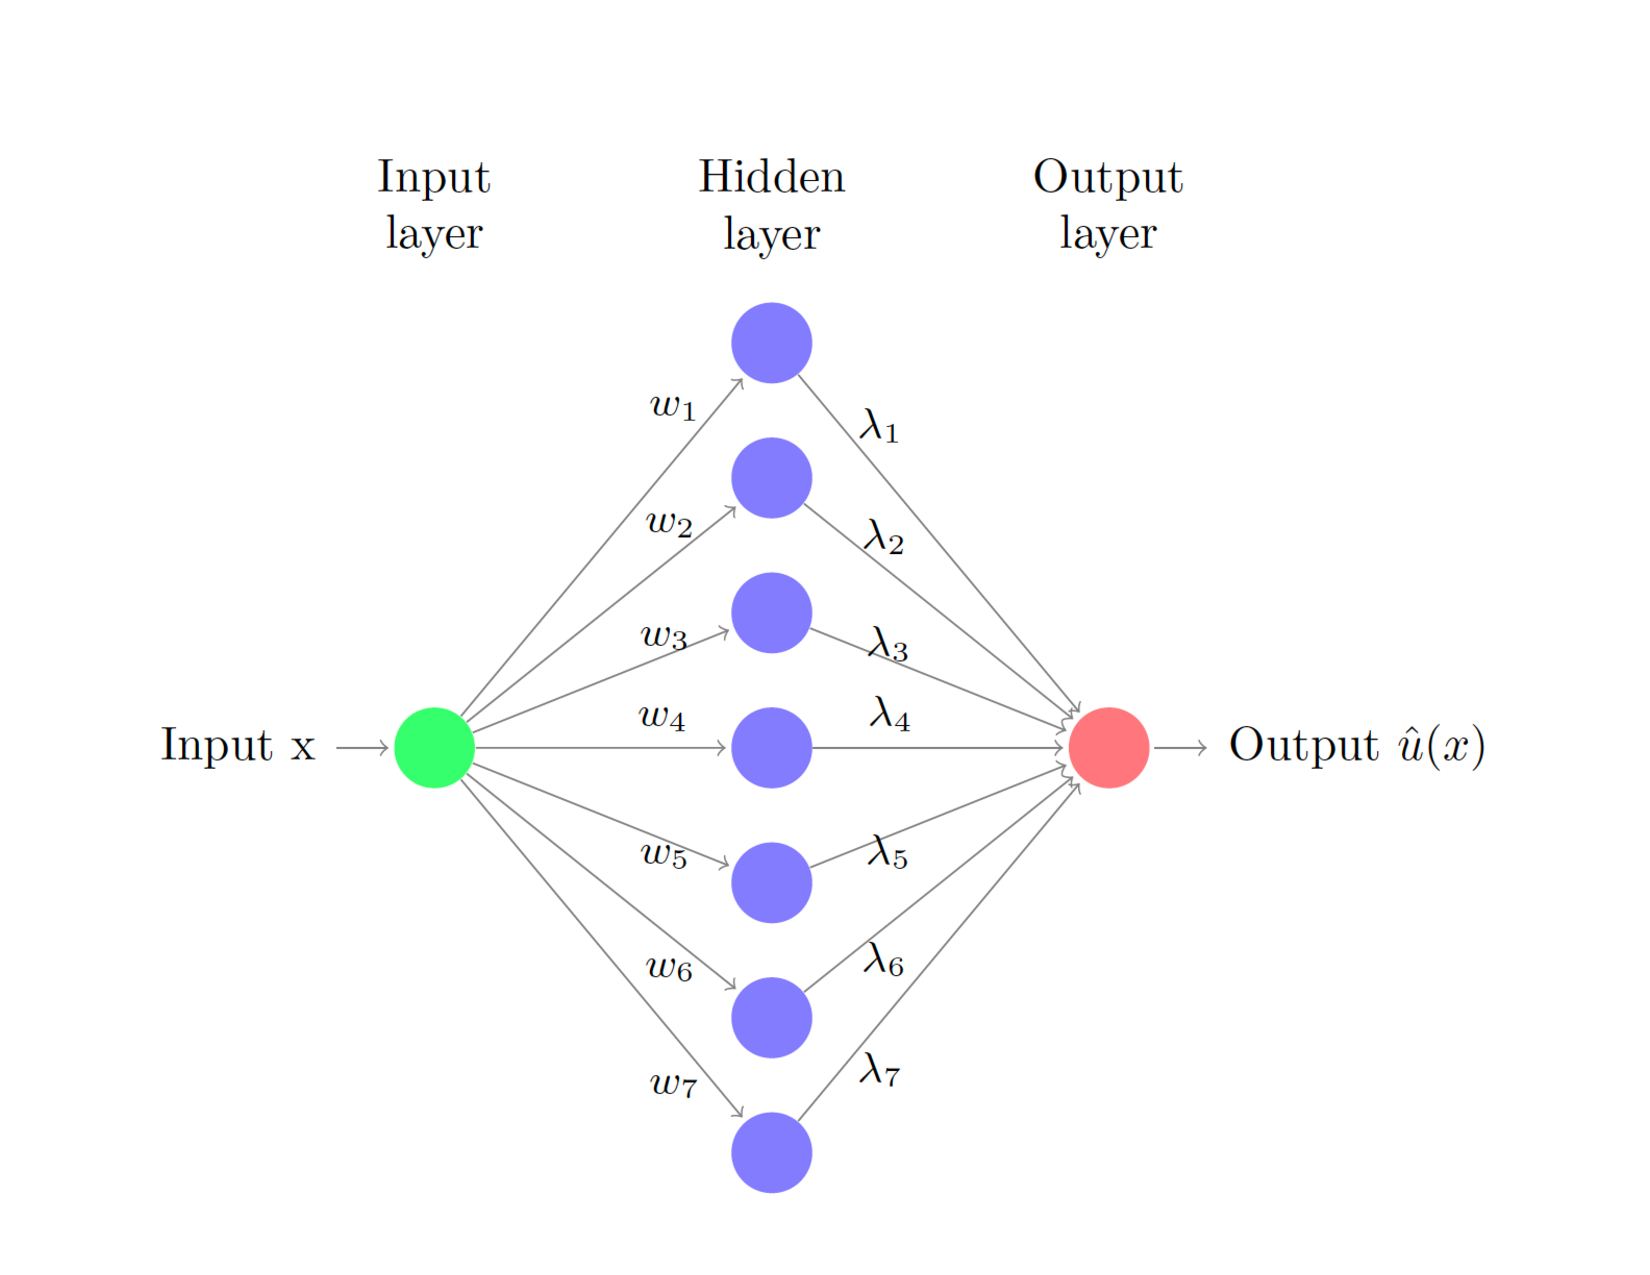
\includegraphics[width=0.6\textwidth]{nn1.pdf}
    \caption{\;Fully connected neural network with a single hidden layer and a one-dimensional input $x \in \mathbf{R}$}
    \label{fig:NN_single}
\end{figure}


On the other end, the Fourier series representation $S_N u$ of a T-periodic function $u \in L^2(\mathbf R)$ is
\begin{equation}\label{Eq: fourier}
    S_{N}u(x) = \frac{a_0}{2} + \sum_{n=1}^N a_{n} \cos(n \omega  x) + b_{n} \sin(n \omega  x) 
\end{equation}
where $x \in [-\frac{T}{2}, \frac{T}{2}]$ $\omega = \frac{2\pi}{T}/$ and $a_{n}$ and $b_{n}$ the Fourier coefficients of $u$. It can be rewritten in the following reduced (phase shift) form:
 \begin{equation}\label{Eq: fourier_shift}
     S_N u(x) = \frac{a_0}{2} + \sum_{n=1}^N c_{n} \cos(n \omega  x + \psi_{n})
 \end{equation}
where for $n \geq 1$, $c_{n} = \sqrt{a_{n}^2 + b_{n}^2}$ and $\psi_n = \arctan2(-\frac{b_{n}}{a_{n}})$. 
% In this work, we only consider one-dimensional cases and reserve two-dimensional cases to future work. In this case, the above expression simplifies to:

%  \begin{equation}\label{Eq: fourier_shift_1d}
%      S_N u(x) = \frac{a_0}{2} + \sum_{n=1}^N c_{n} \cos(n \omega x + \psi_{n})
%  \end{equation}
Therefore, by taking the activation function to be the function $x \mapsto \cos(\omega x)$ in equation (\ref{Eq: NN1d}), one obtains a formulation equivalent to the Fourier decomposition. The input to hidden layer weights $w_k$ mimic the nodes $n$, the hidden layer to output weights $\lambda_k$ approximate the Fourier coefficients $c_n$, the biases of the hidden layer $\phi_k$ correspond to the phase shifts $\psi_k$ and the bias of the output $\phi_0$ to half the $0th$ order Fourier coefficients $a_0$. However as we empirically show below, the equivalency is not straightforward and one needs to train the network with a specific loss function in order to obtain satisfactory results. In the rest of this paper, we restrict ourselves to $2$-periodic function which means the activation function is $x \mapsto \cos(\pi x)$.
% Barron (\cite{Barron}) has proved that any function could be approximated by a single layer neural network with sigmoidal activation functions i.e with an activation function $\sigma$ s.t $\sigma(x) -> 0$ when $x -> -\infty$ and $\sigma(x) -> 1$ when $x -> \infty$. Leshno et al. \cite{Leshno} have proved that multilayer feedforward (define) networks with a nonpolynomial activation function can approximate any function. \\

% Here, we make use of the Fourier representation  of a T-periodic function $u$ $L^2(\mathbf R^M)$ and use the cosine function as the activation function of our network. $S_N u$ is defined as
% \begin{equation}\label{fourier}
%     S_{N}u(x) = \sum_{\nu \in \mathbf{N}^M, \nu_{i}\leq N} a_{\nu} \cos(\omega (\nu\cdot x)) + b_{\nu} \sin(\omega(\nu\cdot x)) 
% \end{equation}
% where $\omega = 2\pi/T$ and $a_{\nu}$ and $b_{\nu}$ the Fourier coefficients of $u$. In the rest of the paper, we restrict ourselves to the one-dimensional case so that the Fourier approximation is

% If we define for $n \geq 1$ $c_{\nu} = \sqrt{a_{\nu}^2 + b_{\nu}^2}$ and $\psi_n = arctan2(-b_{nu}/a_{\nu})$, we can rewrite the above decomposition as
% \begin{equation}\label{fourier_shift}
%     S_N u(x) = \frac{a_0}{2} + \sum_{\nu \in \mathbf{N}^M, \nu_{i}\leq N} c_{\nu} \cos(\omega (\nu\cdot x) + \psi_{\nu})
% \end{equation}
%\subsection{The one dimensional case}


\subsection{Loss function}
The goal of our network is to approximate the Fourier approximation $S_N u$ of $u$. To that end, we define the loss function as
 \begin{equation}\label{Eq:lossfunction}
     L(\phi, w, \lambda) = ||\hat{u} - u ||_2^2  + \alpha_1||\lambda||^2 + \alpha_2||w||^2
 \end{equation}
 where
 \begin{enumerate}
     \item The first term $ ||\hat{u} - u ||_2^2$ ensures that the output of the neural network approximates the target function $u$,
     \item The second $\alpha_1||\lambda||^2$  and third $\alpha_2||w||^2$ terms are regularization terms to avoid overfitting of the Neural Network. Choosing a $L^2$ norm for the regularization parameters causes the weights to decay asymptotically to zero, while a $L^1$ regularization might decrease them to exactly zero. We keep the choice of the regularization for section \ref{subsec:results}.
 \end{enumerate}
 
 However, this loss function will not provide an approximation of the Fourier series of a desired function unless that function is exact combination of cosines or sines. For example, fitting $u(x) = x^2$ with one neuron in the hidden layer led to the output 
 $$\hat{u}(x) = \phi_0 - \lambda_1 \cos(\pi w_1 x)$$ where  $\frac{\lambda_1 \pi^2 w_1^2}{2!} \approx 1$, $\lambda_1 \approx \phi_0 \approx 1$ and $(\pi w_1)^{2l} << 1$ for $l >1$. While this, using the fact that
 $$
 \cos(\pi w_1 x) = \sum_{l=1}^{\infty} (-1)^l\frac{(\pi w_1)^{2l}x^{2l}}{(2l)!} = 1 -\frac{\pi^2 w_1^2}{2!}x^2 + o(w_1^3)
 $$
 or equivalently
  $$
 x^2 \approx ( \cos(\pi w_1 x) - 1 )\frac{2!}{\pi^2 w_1^2} \approx \phi_0 - \lambda_1 \cos(\pi w_1 x)
 $$
 is a good approximation of $x^2$, is not the desired output. To obtain the Fourier representations of the target functions, the weights from the input to the hidden layer need to be approximately integers. This can be achieved by solving a mixed integer optimization problem which is out of the scope of this paper or by modifying the loss function as follows
  \begin{equation}\label{Eq:lossfunction_good}
     L(\phi, w, \lambda) = ||\hat{u}(x) - u(x) ||_2^2  + \alpha_1||\lambda||^2 + \alpha_2||w||^2 + \alpha_3\left( ||\hat{u}(x + T) - \hat{u}(x)||_2^2 \right)+ \alpha_4 \left( ||\hat{u}(x - T) - \hat{u}(x)||_2^2 \right)
 \end{equation}
This amounts to forcing the output of the neural network to be periodic and is equivalent to the input to hidden layer weights being approximately integers.
% \begin{theorem}
% \textcolor{red}{need writing in terms of the nodes captured by the FNN and $S_{max of those nodes}u$}\\
% Let $u$ \in $L^2(\mathbf R^M)$ be a $T$-periodic function. Then, if we denote by $\hat{u}$ the output of the constructed FNN, we have the following bounds on the approximation:
% \begin{itemize}
%     \item If $u$ is analytical, then $||\hat{u}(x) - u(x) ||_2^2 \le C_1 f_1(N) $ 
%     \item If $u$ is piecewise analytical, then $||\hat{u}(x) - u(x) ||_2^2 \le C_2 f_2(N) $,
% \end{itemize}
% \end{theorem}
% \begin{proof}
% If $u$ is analytical, then 
% $$||\hat{u}(x) - u(x) ||_2^2 \le ||\hat{u}(x) - S_N u(x) ||_2^2 + ||S_N u(x) - u(x) ||_2^2$$
% \textcolor{red}{to be completed}
% \end{proof}



\subsection{Weights and biases initialization}\label{subsec:weightsini}
%\color{red} This part I am rewriting, the first part in particular, I need more reading to avoid 'big statements' that would raise eyebrows, didnt touch it for a while\color{black}
A proper weight initialization can significantly improve the performance of a neural network in the training phase specially when dealing with DNNs. In fact, when training DNNs, one is often faced with the vanishing/exploding gradients phenomenon \cite{Geron2017} which causes the training to not converge to a good solution. Here, even though we have a shallow NN, initialization is important to speed up the training. The authors in \cite{Glorot2010} have proposed an initialization method when using the logistic activation function that circumvent that issue. In essence, they proved that one needs the variance of the outputs of each layer to be equal to the variances of its inputs. Furthermore, the variances of the gradients should be equal before and after going through a layer in the reverse direction. \cite{Heinit2015} proposed an initialization strategy for the ReLU activation function. In \cite{Kumar2017}, the author extended this result to nonlinear activation functions differentiable at $0$. We propose below an initialization strategy for the FNN presented here. As it is commonly the case, we initialize the biases to $0$. In what follows, we use a few properties of the mean and variance of a random variable that are recalled in appendix \ref{appendixA}. We denote by $X$ a random variable to differentiate it from its realization $x$. \\
Let $x$ be the input of our FNN and $\{x_k\}_{k = 1..N}$ the hidden layer nodes (see figure \ref{fig:NN_single}). For the sake of simplicity, we denote by $y$ the output of the network instead of $\hat{u}(x)$ in this section. . Then, as the biases are equal to $0$,
$$
x_k = \cos(\pi w_k x ) \;\; \text{and}\;\; y = \sum_{k = 1}^N \lambda_k \cos(\pi w_k x). 
$$

% $\{x_{j0}\}_{j0 = 1..M}$
 We assume that the input $x$ of the FNN is a vector of size $M$ whose elements were drawn uniformly in $[-1 \;\; 1]$. That means (see appendix \ref{appendixA}) that $$\mu(X) = 0  \;\; \text{and}\;\; \sigma^2(X) = \frac{1}{3}. $$ where $\mu(X)$ denotes the mean of a random variable $X$ and $\sigma^2(X)$ its variance defined by
 \begin{align*}
     \mu(X) &= \int_{-\infty}^{+\infty} xf(x) dx \\
     \sigma^2(X) &= \mu(X^2) - \left(\mu(X)\right)^2
 \end{align*}


 
%Therefore, the expected value of $x$ is 
% $$
% \mu(x) = [0, \cdots, 0]^T
% $$
% and  its covariance matrix
% $\Sigma(x) = $\[
%   \begin{pmatrix}
%     1/3 & 0 & \dots & 0 \\
%     0 & 1/3 & \dots & 0 \\
%     \vdots & \vdots & \ddots & \vdots \\
%     0 & 0 & \dots & 1/3
%   \end{pmatrix}
% \]


Furthermore, we assume the weights $w_k$ are drawn from a normal distribution $\mathcal N(0, m^2)$ and the weights $\lambda_k$ are drawn from a normal distribution $\mathcal N(0, v^2)$. The goal is to find values of $m$ and $v$ such that the variances at each of the layers of the network are equal during the first forward pass i.e $$\sigma^2(X) = \sigma^2(X_k) = \sigma^2(Y),\; \; \forall k=1\cdots N$$.
\begin{enumerate}
    \item \textbf{Initializing the input layer to hidden layer weights  $\mathbf{w_k}$}: 
    % $$\mu(w_k x) = 0 \;\; \text{and}\;\; \sigma^2(w_k x) = m^2/3.$$
    We first compute the mean of the node $k$ of the hidden layer. To that aim, we use the following theorem called the Law Of The Unconscious Statistician (LOTUS).
\begin{theorem}
Let X, Y be continuous random variables with a joint density function $f_{(X,Y)}$ and h be a continuous function of two variables such that
$$\int_{\mathbf{R^2}} |h(x,y)| f_{(X,Y)}(x,y) dx dy < +\infty,\;\; \text{then, we have}$$
$$\mu\left(h(X,Y)\right) = \int_{\mathbf{R^2}} h(x,y) f_{(X,Y)}(x,y) dx dy  $$
\end{theorem}

Therefore, knowing that the joint probability distribution of the two independent random variables $W_k$ and $X$ is $f_{(W_k,X)}(x,y) = \frac{1}{2} \cdot \frac{1}{w \sqrt{2\pi}} e^{\frac{-w_k^2}{2m^2}}$, we obtain (using $h(w_k,x) = \cos(\pi w_k x)$ in the above theorem) 
\begin{equation}\label{Eq:muxk}
    \mu(X_k) = \mu(\cos(\pi W_k X)) = \int_{-1}^{1} \int_{-\infty}^{+\infty}\frac{1}{2} \cos(\pi w_k x)\frac{1}{w \sqrt{2\pi}} e^{\frac{-w_k^2}{2m^2}}\; dw_k dx.
\end{equation}
Let $I_1 = \int_{-\infty}^{+\infty} \cos(\pi w_k x)\frac{1}{m \sqrt{2\pi}} e^{\frac{-w_k^2}{2m^2}}\; dw_k$, then, using integration by parts, we obtain
$$I_1 = \frac{|m|}{m}e^{-\frac{1}{2}m^2x^2} = e^{-\frac{1}{2}m^2x^2}. $$
This means
$$ \mu(X_k) = \int_{-1}^{1}\frac{1}{2} e^{-\frac{\pi}{2}m^2x^2} dx $$
which gives

\begin{equation}\label{Eq:muxk_last}
    \mu(X_k) = \frac{1}{m\sqrt{2\pi}}erf\left(\frac{m\pi}{\sqrt{2}}\right) 
\end{equation}
where $erf$ is the error function.\\
Now, to compute the variance of $X_k$, we recall that
$$\sigma^2(X_k) = \mu(X_k^2) - (\mu(X_k))^2.$$ 
We then use the trigonometric identity $$x_k^2 = \cos^2(\pi w_k x) = \frac{1}{2} + \frac{\cos(2\pi _kx)}{2}$$ which leads to
\begin{equation*}
    \mu(X_k^2) = \int_{-1}^{1}\frac{1}{2} \int_{-\infty}^{+\infty} \frac{1}{2}(1 + \cos(2 \pi w_k x))\frac{1}{m \sqrt{2\pi}} e^{\frac{-w_k^2}{2m^2}}\; dw_k dx
\end{equation*}
After integration, we obtain 
$$\mu(X_k^2) = \frac{1}{2} + \frac{1}{4\sqrt{2\pi}}\frac{erf\left(\sqrt{2}m\pi\right)}{m}.$$
Put together, the variance of $X_k$ becomes
\begin{equation}\label{Eq:varxk_last}
    \sigma^2(X_k) = \frac{1}{2} + \frac{1}{4\sqrt{2\pi}}\frac{erf(\sqrt{2}m\pi)}{m}-\left(\frac{1}{m\sqrt{2\pi}}erf\left(\frac{m\pi}{\sqrt{2}}\right) \right)^2 .
\end{equation}
Because we want the variance of the output of the hidden layer to be equal to the variance of its input i.e $$\sigma^2(X_k) = \sigma^2(X) = \frac{1}{3}, $$ we need to solve 
\begin{equation*}
    \frac{1}{3} = \frac{1}{2} + \frac{1}{4\sqrt{2\pi}}\frac{erf(\sqrt{2}m\pi)}{m}-\left(\frac{1}{m\sqrt{2\pi}}erf\left(\frac{m\pi}{\sqrt{2}}\right) \right)^2 .
\end{equation*}
which admits a unique solution $m \approx 0.6959$. However, this value being small, this means that imposing this type of initialization on the hidden layer weights will cause the FNN to capture fewer Fourier modes than we are seeking. Therefore, we initialize these weights using a normal distribution $\mathcal N(0,5)$ which means $m = \sqrt{5}$. This value was picked by trial and error and as showed in the results section \ref{subsec:results}, allows us to recover the first 5 Fourier nodes of a periodic function. Plugging in $m$ in equation (\ref{Eq:varxk_last}) gives
$$\sigma^2(X_k) \approx .5128$$. 
    
    \item \textbf{Initializing the hidden layer to output layer weights  $\mathbf{\lambda_k}$}: Now, for the output $y$, since $\Lambda_k$ and $\cos(W_k X)$ are independent, we can write $$\mu(Y) = \sum_{k = 1}^N \mu(\lambda_k) \mu(\cos(w_k x  ))$$ and $$\sigma^2(Y) = \sum_{k = 1}^N \sigma^2 (\Lambda_k)  \left(\sigma^2\left(\cos(W_k X)\right)+\mu^2\left(\cos(W_k X)\right) \right) +  \mu^2(\Lambda_k)\sigma^2\left(\cos(W_k X)\right)$$ 
    where $\sigma^2 (\Lambda_k) = v^2$ and $\mu(\Lambda_k) = 0$. This leads to
\begin{equation}\label{Eq:vary}
    \sigma^2(Y) = N\left[ v^2\left[\frac{1}{2} + \frac{1}{4\sqrt{2\pi}}\frac{erf\left(\sqrt{2}m\pi\right)}{m}\right] \right].
\end{equation}
Since we want $\sigma^2(Y) = \sigma^2(X_k) \approx .5128$, we get 
\begin{equation}\label{Eq:varweight2}
    v^2 = \frac{0.5128}{N\left(\frac{1}{2} + \frac{1}{4\sqrt{2\pi}}\frac{erf\left(\sqrt{2}m\pi\right)}{m}\right)} 
\end{equation}
where $m = \sqrt{5}$.
\end{enumerate}





\subsection{Results}\label{subsec:results}
In this section, we run numerical simulations to assess the effectiveness of the method presented above. We first approximate analytic $2$-periodic functions which are linear combinations of sines and cosines. High accuracy is expected on such functions due to the way the FNN was built. Then, we aim at recovering low-frequency Fourier coefficients of piecewise analytic periodic functions. These functions are of particular interest since they are very common in fields like acoustics or electronics.
\subsubsection{Analytic Periodic Functions}
In order to investigate the performance of the above constructed network, we first attempt to approximate the 2-periodic function 
 $$
 f(x) = \cos(\pi x) + \sin(\pi x)\;.
 $$
 with four nodes in the hidden layer. We show results for both $L^2$ and $L^1$ regularizations.
We report the parameters of the network upon convergence in tables (\ref{tab:tabcossinL2}-\ref{tab:tabcossinL1}) along with the number of iterations and the value loss function. We notice that the output of the FNN is
$$\hat{u}(x) \approx \sqrt{2}\cos(\pi x - \frac{\pi}{4})$$ 
which is the reduced form of  $f(x)= \cos(\pi x) + \sin(\pi x)$. The optimization converged to approximately $2e-4$ in $189$ iterations for the $L^2$ regularization against $3e-4$ in $87$ iterations for the $L^1$ one. Although the results for the $L^1$ regularization are slightly better, none of the hidden layer to output weights converged to exactly zero as was expected.

 \begin{table}[!h]
  \begin{center}
\begin{tabular}{ |c|c|c|c|c| } 
  \hline
  \multicolumn{3}{|c|}{Number of iterations} & $189$  \\
\hline
  \multicolumn{3}{|c|}{Loss Function (upon convergence)} & $2e-4$  \\
\hline
\hline
$w_k$ & $\phi_k$ & $\lambda_k$& $\phi_0$ \\
\hline
$1.00000000$ & $-0.78539816 \approx -\pi/4$ &$1.41421354 \approx \sqrt{2}$& \\ 
$-5.96856597e-07$&$-1.00911547$ & $-2.60499122e-05$& $-1.81893539e-05$ \\ 
$1.22755482e-06$& $1.87773726$ & $-4.76966579e-05$& \\ 
$4.59348246e-08$& $-6.38405893 $ & $1.77429347e-05$& \\ 
\hline
\end{tabular}
\caption{\;Number of iterations, value of the loss function at convergence and optimal weights and biases of the FNN to approximate $ f(x) = \cos(\pi x) + \sin(\pi x)$, $k = 1\cdots4$ with a $L^2$ regularization.}\label{tab:tabcossinL2}
\end{center}
\end{table}

 \begin{table}[!h]
  \begin{center}
\begin{tabular}{ |c|c|c|c|c| } 
  \hline
  \multicolumn{3}{|c|}{Number of iterations} & $87$  \\
\hline
  \multicolumn{3}{|c|}{Loss Function (upon convergence)} & $3e-4$  \\
\hline
\hline
$w_k$ & $\phi_k$ & $\lambda_k$& $\phi_0$ \\
\hline
$1.00000033$ & $-0.78540193 \approx -\pi/4$ &$1.41421847 \approx \sqrt{2}$& \\ 
$1.4969094$&$-0.71483098$ & $-4.32639025e-06$& $1.58219741e-05$ \\ 
$0.05095418$& $ 0.96613253$ & $6.73308554e-05$& \\ 
$0.14126515$& $-5.84166681 $ & $-5.13186621e-05$& \\ 
\hline
\end{tabular}
\caption{\;Number of iterations, value of the loss function at convergence and optimal weights and biases of the FNN to approximate $ f(x) = \cos(\pi x) + \sin(\pi x)$, $k = 1\cdots4$ with a $L^1$ regularization. }\label{tab:tabcossinL1}
\end{center}
\end{table}

 \begin{figure}[!htb]
    \centering
    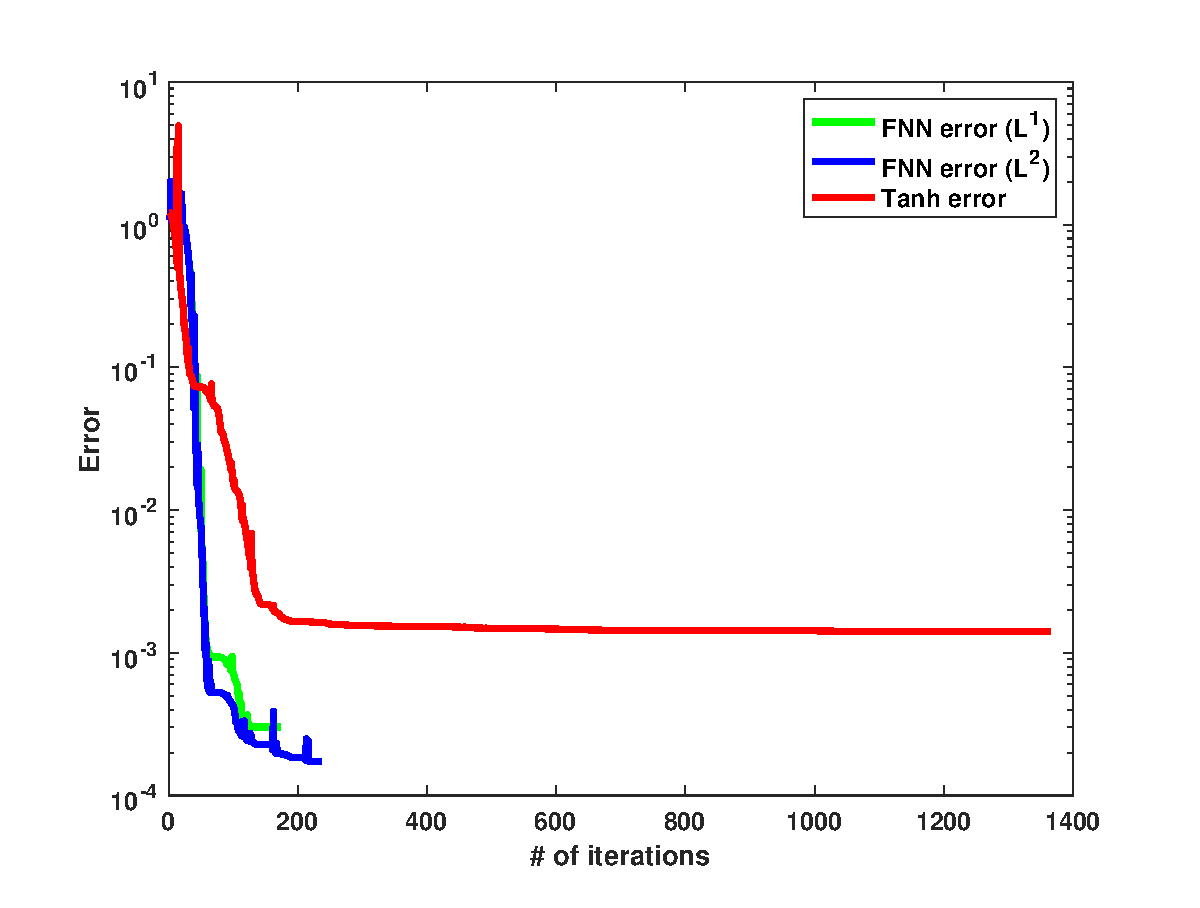
\includegraphics[width=0.45\textwidth]{itertanhvsfnn.eps}
    \caption{\;Comparison in terms of the values of the loss function throughout the optimization when using a FNN and when using a neural network with a $\tanh$ activation.}
    \label{fig:fourvsNN_iter}
\end{figure}


We compare in figure (\ref{fig:fourvsNN_iter}) the performances of the above constructed FNN and of a regular neural network with a $\tanh$ activation function and a Glorot initialization \cite{Glorot2010}. The latter network converged to approximately $1e-3$ in $1173$ iterations which showcases the significant gain in iteration number obtained when using the FNN. The error is also improved by an order of $10$ with the FNN. To further illustrate the advantages of using the presented FNN, we display in figure (\ref{fig:fourvsNN_outside}) a significant benefit it has. In fact, it also produces a good approximation of the desired function outside of the training domain. A major shortcoming of neural networks methods for function approximation is indeed their inability to preserve the sought function outside of the training region. The architecture presented here is able to overcome that issue due to the way the loss function was defined in equation (\ref{Eq:lossfunction_good}). It is worth noting that we did not include the periodicity requirement in the loss function when training the traditional neural network, the results were worst in that it required more nodes in the hidden layer, convergence was reached more slowly and the error was similar.

%  \begin{figure}[!htb]
%     \centering
%     \subfigure{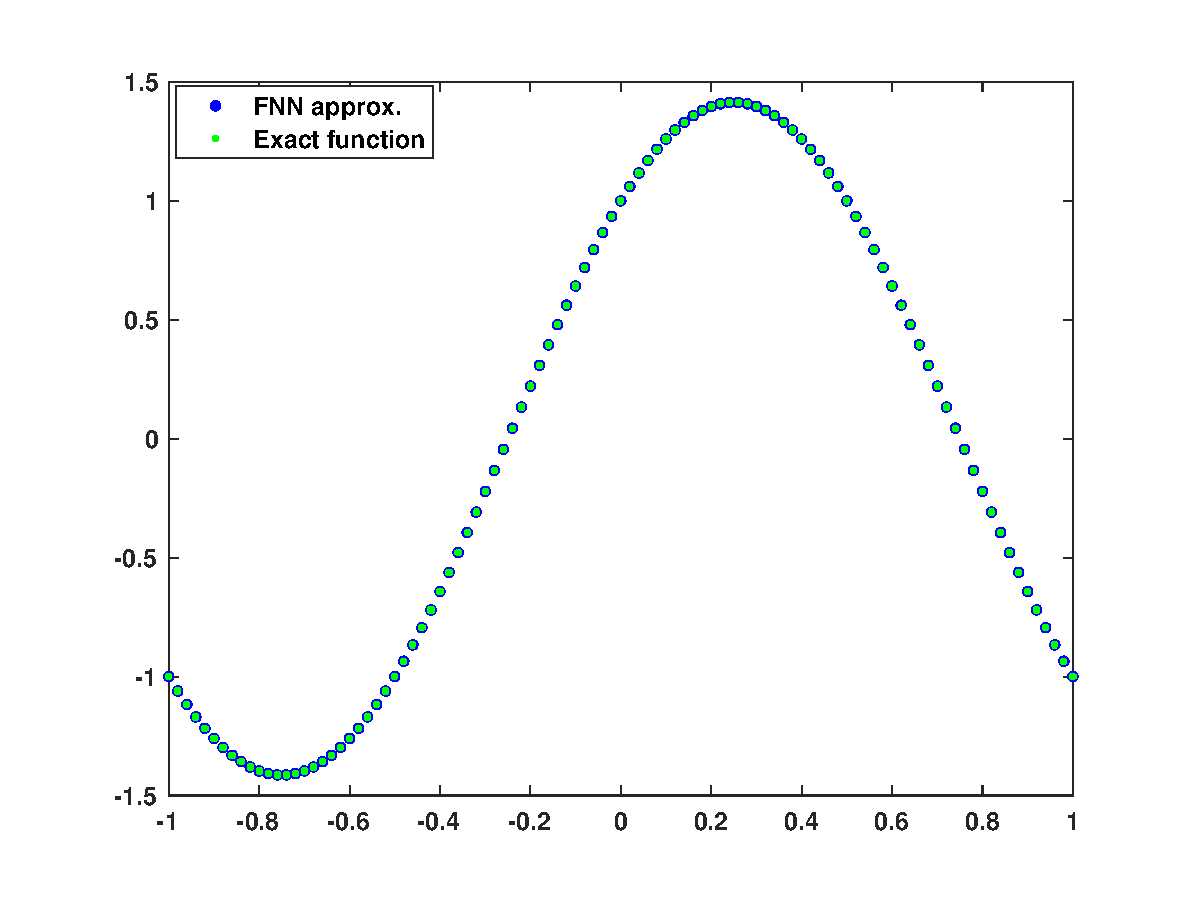
\includegraphics[width=0.45\textwidth]{FNNcossinnodes4.eps}}
%     \subfigure{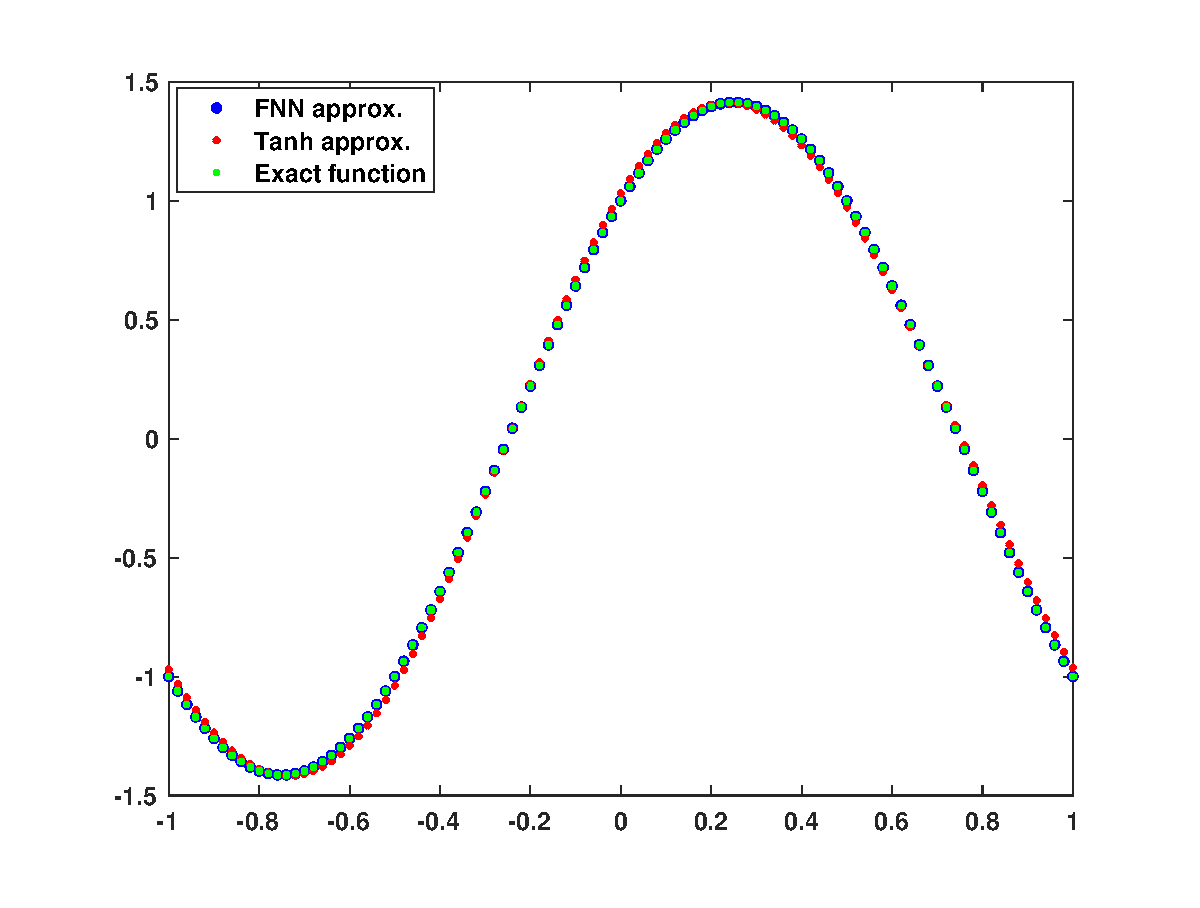
\includegraphics[width=0.45\textwidth]{FNNvstanhsincos.eps}}
%     \caption{(Top)Comparison between the approximation obtained by our Fourier Neural Network and the exact solution. (Bottom)Comparison between the approximation obtained by using a tanh activation function and the exact solution}
%     \label{fig:fourvsNN_percs}
% \end{figure}


 
   \begin{figure}[!htb]
    \centering
    \subfigure{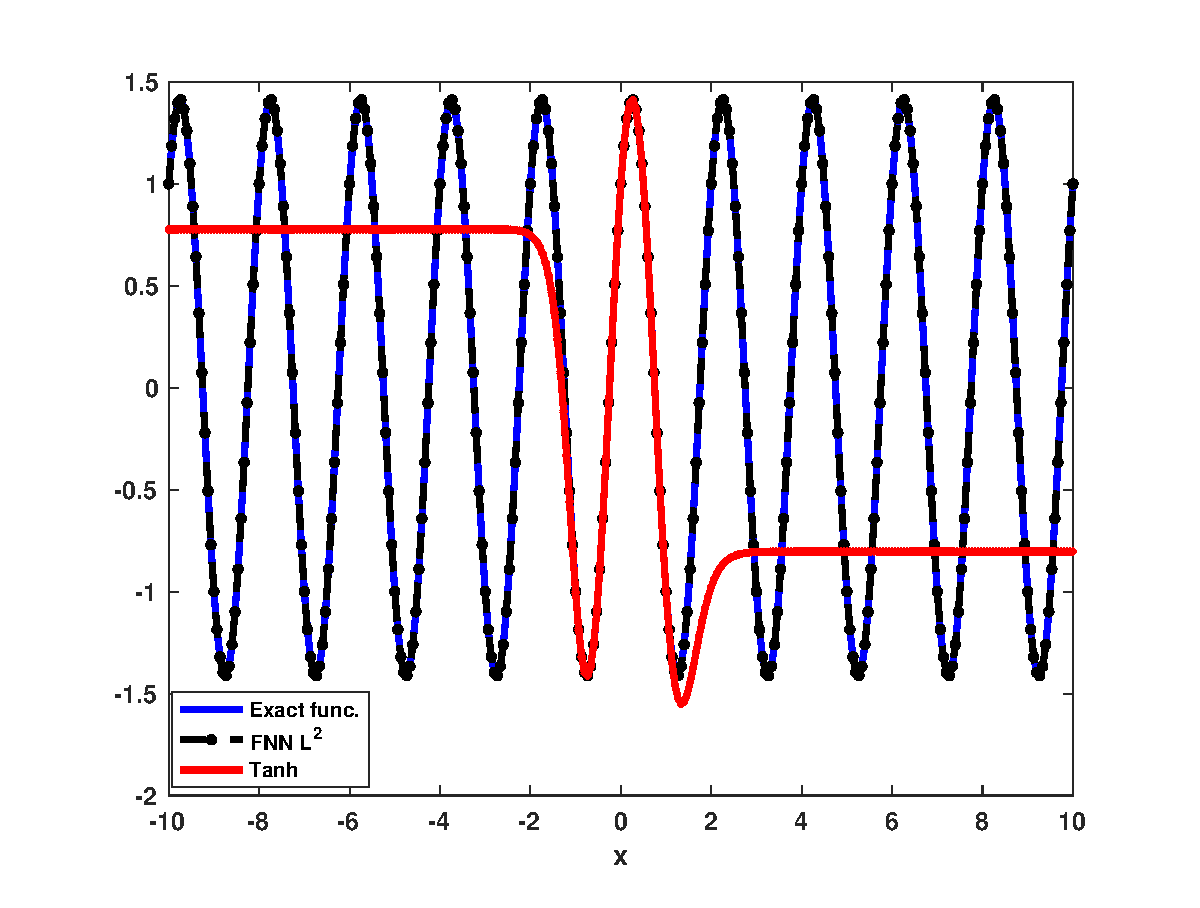
\includegraphics[width=0.45\textwidth]{fnnl2vstanhoutside.eps}}
     \subfigure{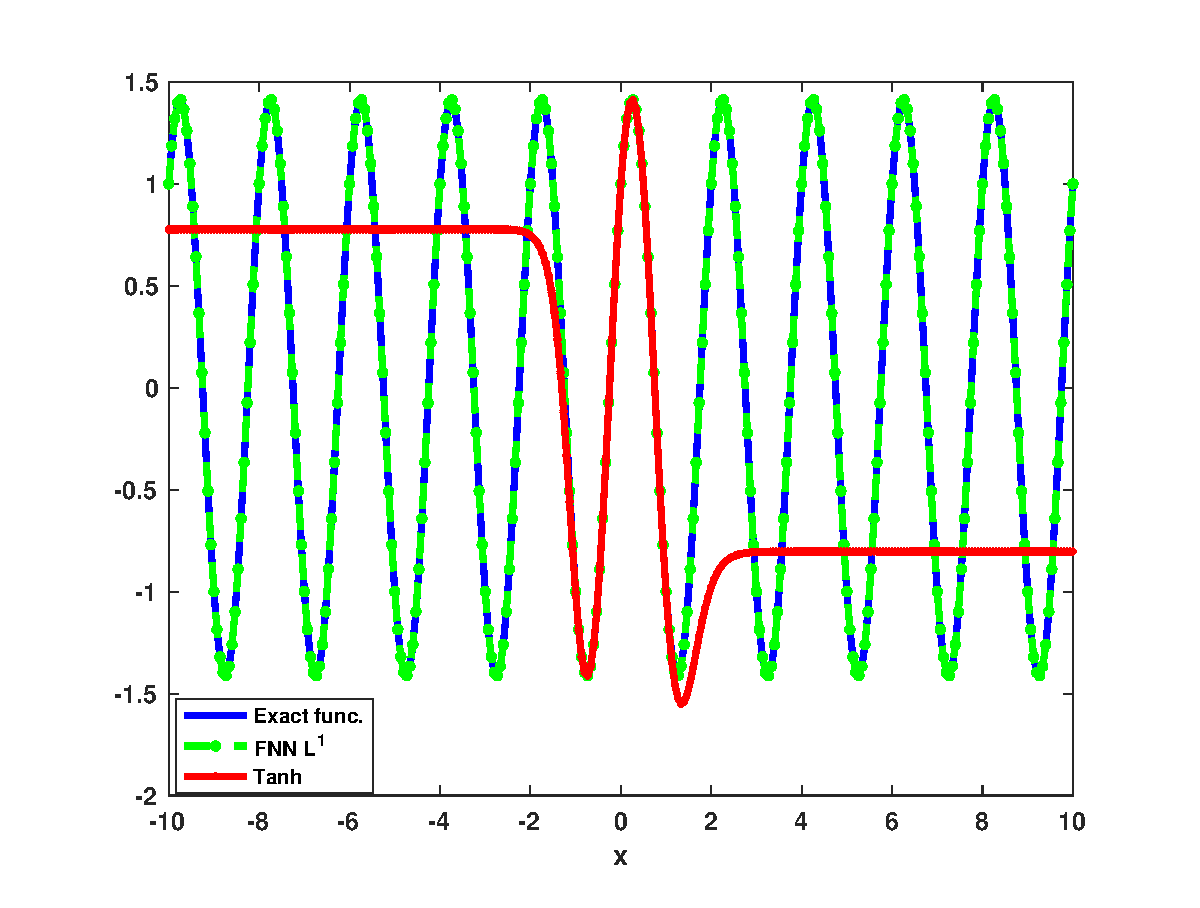
\includegraphics[width=0.45\textwidth]{fnnl1vstanhoutside.eps}}
    \caption{\;Comparison between $f(x) = \cos(\pi x) + \sin(\pi x)$ and the output of the FNN  outside of the training domain for both $L^2$ (left) and $L^1$ (right) regularizations}
    \label{fig:fourvsNN_outside}
\end{figure}


We then seek to estimate the function 
$$g(x) = 8 \cos(4\pi x) + \sin(2\pi x) + \sin(\pi x)$$ with the same architecture as above. We show in tables (\ref{tab:tabpercompL2}-\ref{tab:tabpercompL1}) the value of the loss function (error) upon convergence, the number of iterations as well as the values of the weights obtained upon convergence. The optimization converged to approximately $9e-4$ after $195$ iterations when using a $L^2$ regularization on the weights and to approximately $1e-3$ after $169$ iterations when using a $L^1$ one.  We note the biases are approximations of odd multiples of $\pi/2$ for the sine part of the function $g$ and approximately $0$ for its cosine part. 



%   \begin{table}[!h]
%   \begin{center}
%   \begin{tabular}{ |c|c|c| } 
%  \hline
%   &$L^2$ regularization & $L^1$ regularization  \\
%  \hline
%  number of iterations & $195$ &$169$ \\ 
%  \hline
%  Error&$9e-4$ & $1e-3$ \\ 
%  \hline
%  \end{tabular}
%  \caption{\; Convergence results when approximating $ g(x) = 8 \cos(4\pi x) + \sin(2\pi x) + \sin(\pi x)$}\label{tab:convFNNcomp}
%  \end{center}
%  \end{table}
%tanh converged to 3e-2 in 2049 it with 10 nodes
 \begin{table}[!h]
  \begin{center}
  \begin{tabular}{ |c|c|c|c|c| } 
  \hline
  \multicolumn{3}{|c|}{Number of iterations} & $195$  \\
\hline
  \multicolumn{3}{|c|}{Loss Function (upon convergence)} & $9e-4$  \\
\hline
\hline
$w_k$ & $\phi_k$ & $\lambda_k$& $\phi_0$ \\
\hline
$1.00000000$ & $1.57079627 \approx \pi/2$ &$-9.99999993e-01$& \\ 
$5.40604942e-06$&$1.01888743e+01$ & $3.34351764e-06$& $2.41330937e-06$ \\ 
$4.00000000$& $-9.14402304e-10$ & $7.99999983$& \\ 
$ -2.00000000$& $4.71238899 \approx 3\pi/2$ & $-9.99999984e-01$& \\ 
\hline
\end{tabular}
\caption{\;Number of iterations, value of the loss function at convergence and optimal weights and biases of the FNN to approximate $ g(x) = 8 \cos(4\pi x) + \sin(2\pi x) + \sin(\pi x)$ with $L^2$ regularization, $k = 1\cdots4$}\label{tab:tabpercompL2}
\end{center}
\end{table}


 \begin{table}[!h]
  \begin{center}
  \begin{tabular}{ |c|c|c|c|c| } 
    \hline
\multicolumn{3}{|c|}{Number of iterations}& $169$  \\
\hline
  \multicolumn{3}{|c|}{Loss Function (upon convergence)} & $1e-3$  \\
\hline
\hline
$w_k$ & $\phi_k$ & $\lambda_k$& $\phi_0$ \\
\hline
$0.99999306$ & $1.57072838 \approx \pi/2$ &$-1.000141261$& \\ 
$1.99999672$&$7.85406634 \approx 5\pi/2$ & $-9.99825909e-01$& $3.82384745e-05$ \\ 
$3.99999998$& $-1.14376588e-05$ & $7.99989569$& \\ 
$ -0.04032155$& $-2.12089270e+01$ & $1.69927207e-05$& \\ 
\hline
\end{tabular}
\caption{\;Number of iterations, value of the loss function at convergence and optimal weights and biases of the FNN to approximate $ g(x) = 8 \cos(4\pi x) + \sin(2\pi x) + \sin(\pi x)$ with $L^1$ regularization, $k = 1\cdots4$}\label{tab:tabpercompL1}
\end{center}
\end{table}
 \begin{figure}[!htb]
    \centering
    \subfigure{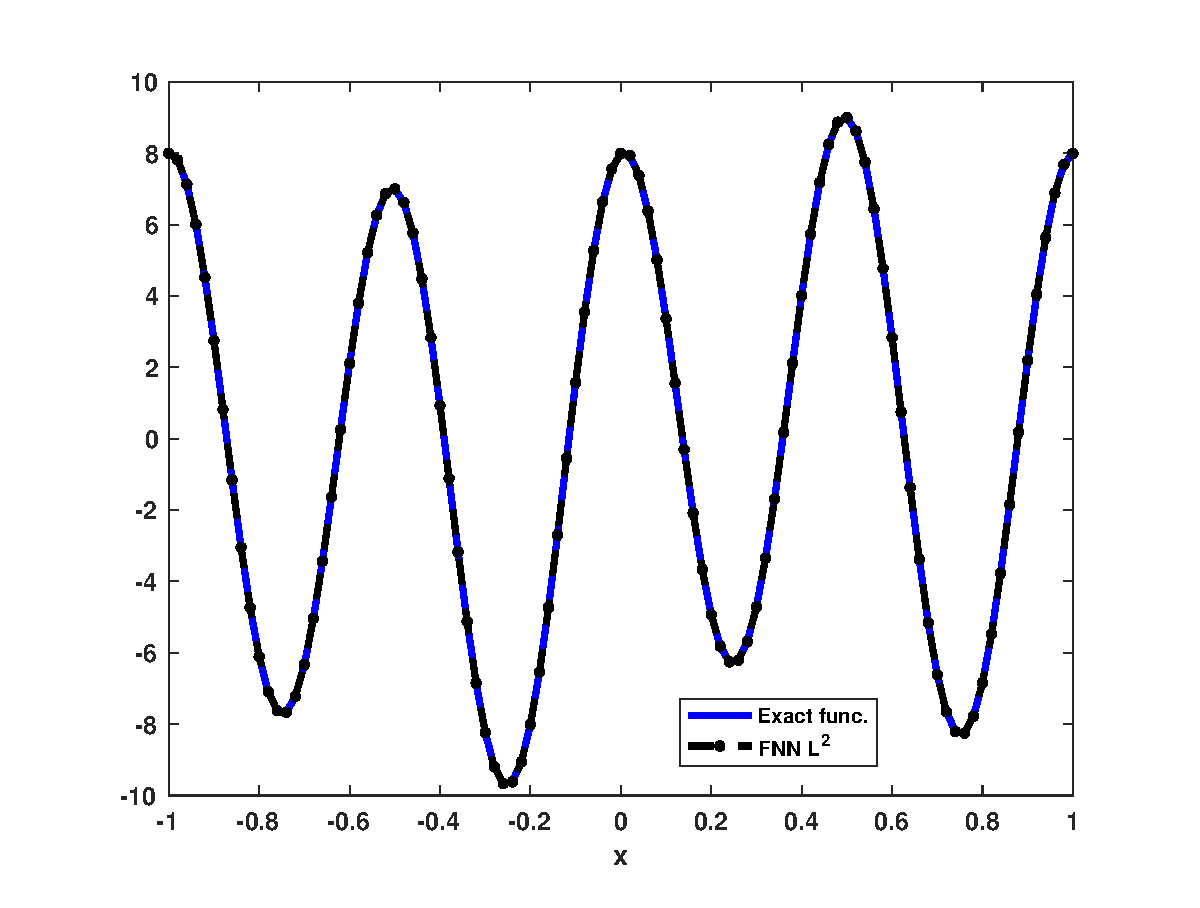
\includegraphics[width=0.45\textwidth]{fnnl2vsexactcomp.eps}}
     \subfigure{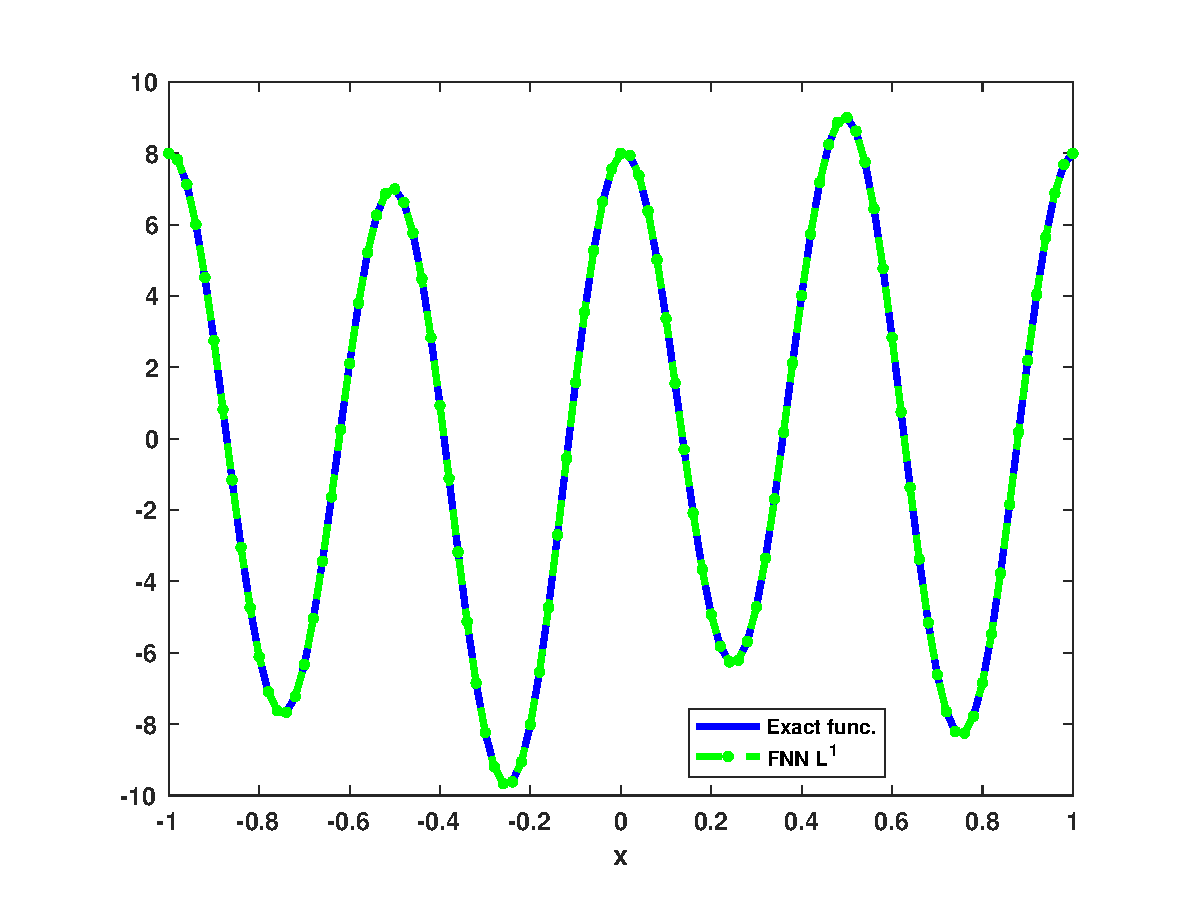
\includegraphics[width=0.45\textwidth]{fnnl1vsexactcomp.eps}}
    \caption{\;Comparison between $g(x) = 8 \cos(4\pi x) + \sin(2\pi x) + \sin(\pi x)$ and the output of the FNN for both $L^2$ (left) and $L^1$ (right) regularizations}
    \label{fig:fourvsNNcompPer}
\end{figure}


We show in figure (\ref{fig:fourvsNNcompPer}) a comparison between the exact function and the approximations provided by the FNN. The actual error between the function and the FNN approximation only is of the order of $1e-8$ for the $L^2$ regularization and $1e-5$ for the $L^1$ one. This, combined with the fact that weights corresponding to redundant node don't go exactly to zero when using $L^1$ regularization, motivates us to use $L^2$ regularization in the rest of the paper. We also compared the FNN approximation to one from a regular neural network with a $\tanh$ activation. The latter converged to a poor local minimum for $4$ nodes in the hidden layer and converged to a value of $3e-2$ for the loss function for $10$ nodes in the hidden layer. 

%(\textcolor{red}{should I add comparison?})




\subsubsection{Piecewise analytic periodic functions}  
Here, we first tried to approximate the non analytical periodic function
\begin{equation}\label{Eq:xsquare}
  f(x) = x^2, \;\; \text{$x \in \left(-(2k+1), (2k+1)\right)$}\;\;, k \in \mathbf{N}  
\end{equation}


We use $4$ nodes in the hidden layer and the FNN captured the first $5$ nodes of the Fourier decomposition (if we count the $0th$ node). We show in table (\ref{tab:tabfnnx2}) the values obtained for the weights and the biases. We call the hidden layer to output weights and the bias of the output layer FNN coefficients. We note that they are $3rd$ order approximations of the Fourier coefficients. Figure (\ref{fig:Fnnx2}) is a good visual representation of the quality of that approximation.
\begin{table}[!h]
  \begin{center}
  \begin{tabular}{ |c|c|c|c|c| } 
    \hline
\multicolumn{3}{|c|}{Number of iterations}& $130$  \\
\hline
  \multicolumn{3}{|c|}{Loss Function (upon convergence)} & $2e-2$  \\
\hline
\hline
$w_k$ & $\phi_k$ & $\lambda_k$& $\phi_0$ \\
\hline
$0.99995578$ & $-0.00477923$ &$-0.40479907$& \\ 
$2.99892898$&$-3.139197051$ & $0.04915202$& $0.335023246$ \\ 
$3.99604127$& $0.01794715$ & $0.02874206$& \\ 
$ -1.99965386$& $0.00445702$ & $ 0.10497063$& \\ 
\hline
\end{tabular}
\caption{\;Number of iterations, value of the loss function at convergence and optimal weights and biases of the FNN to approximate $ f(x) = x^2$ on $[-1, 1$]}\label{tab:tabfnnx2}
\end{center}
\end{table}
The Fourier series of this function is
$$
S(f)(x)= \frac{1}{3} + \sum_{n=1}^{\infty} 4 \frac{(-1)^n}{\pi^2 n^2} \cos(\pi nx)
$$



  \begin{figure}[!htb]
    \centering
    \subfigure{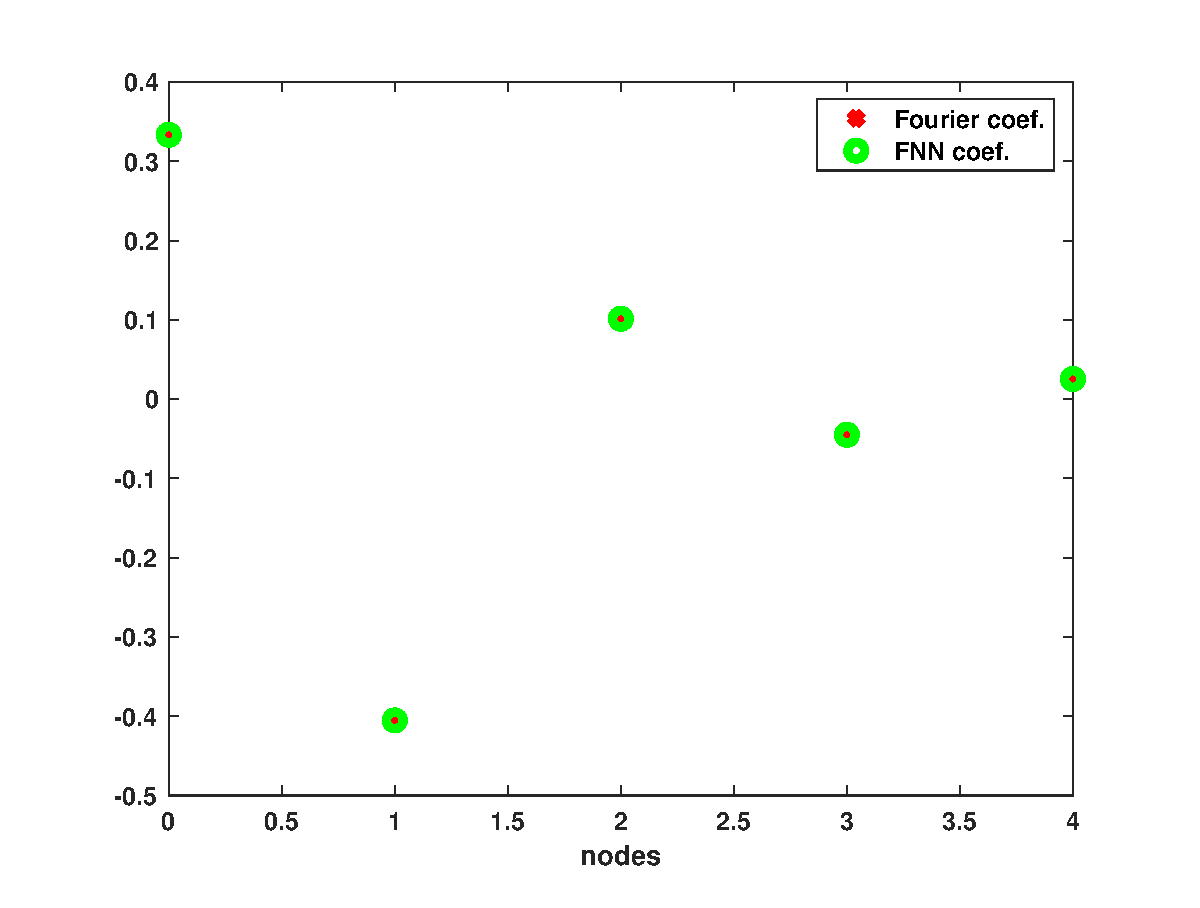
\includegraphics[width=.45\textwidth]{fnncoeffvsfourcoef.eps}}
     \subfigure{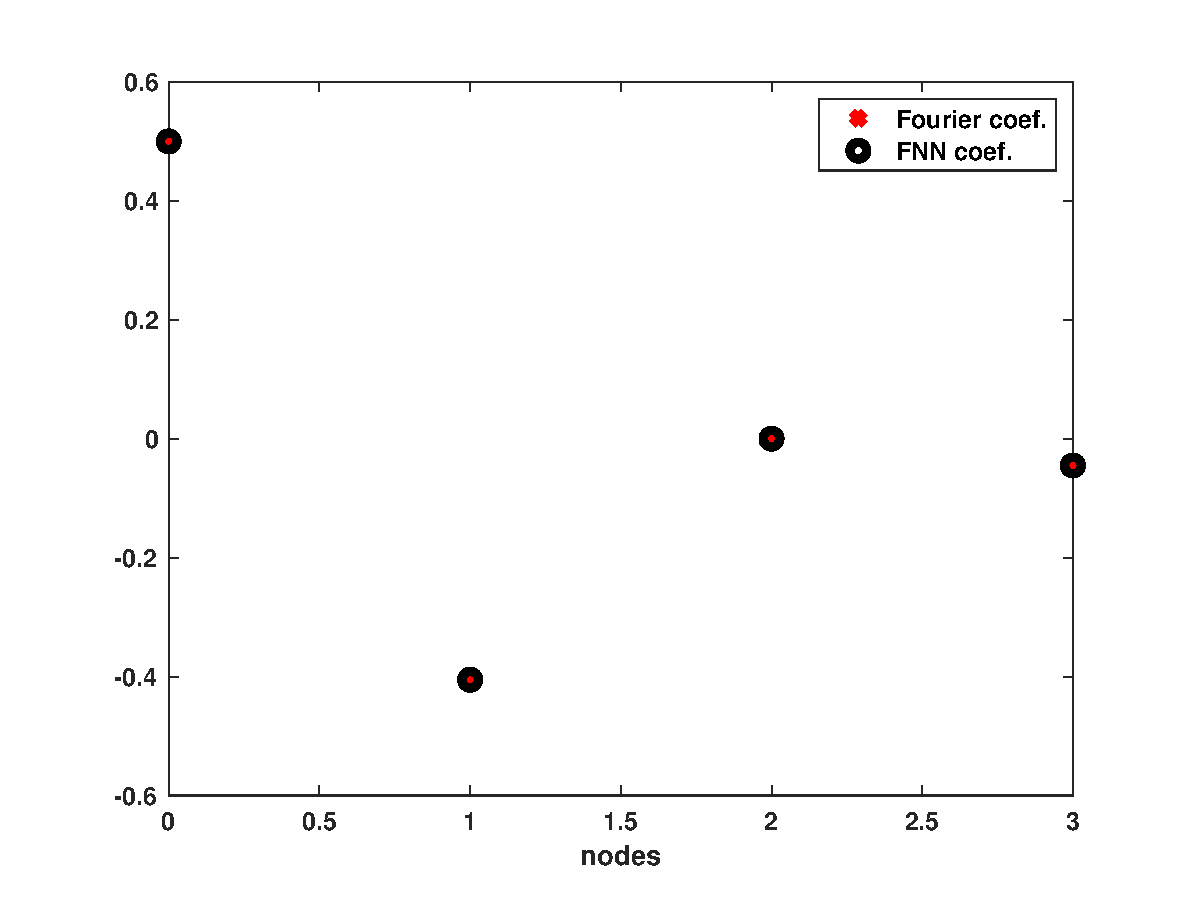
\includegraphics[width=.45\textwidth]{fnncoeffvsfourcoeffabsx.eps}}
    \caption{\;Comparison between the FNN coefficients and the Fourier coefficients of $f(x) = x^2$ (left) and of $g(x) = |x|$ (right) for the nodes captured by the neural network}
    \label{fig:Fnnx2}
\end{figure}
We illustrate in figure (\ref{fig:Fnnx2out}) the behavior of the output of the FNN as opposed to the one from a neural network with a $tanh$ activation function. As expected, the FNN network conserves the  properties of the function to be approximated outside of the training domain while the $tanh$ neural network does not. It is worth noting that the latter was more accurate in this case on the training interval $[-1, 1]$ ($6e-4$ with $3073$ iterations against $2e-2$ with $130$ iterations for the FNN.)
\begin{figure}[!htb]
    \centering
    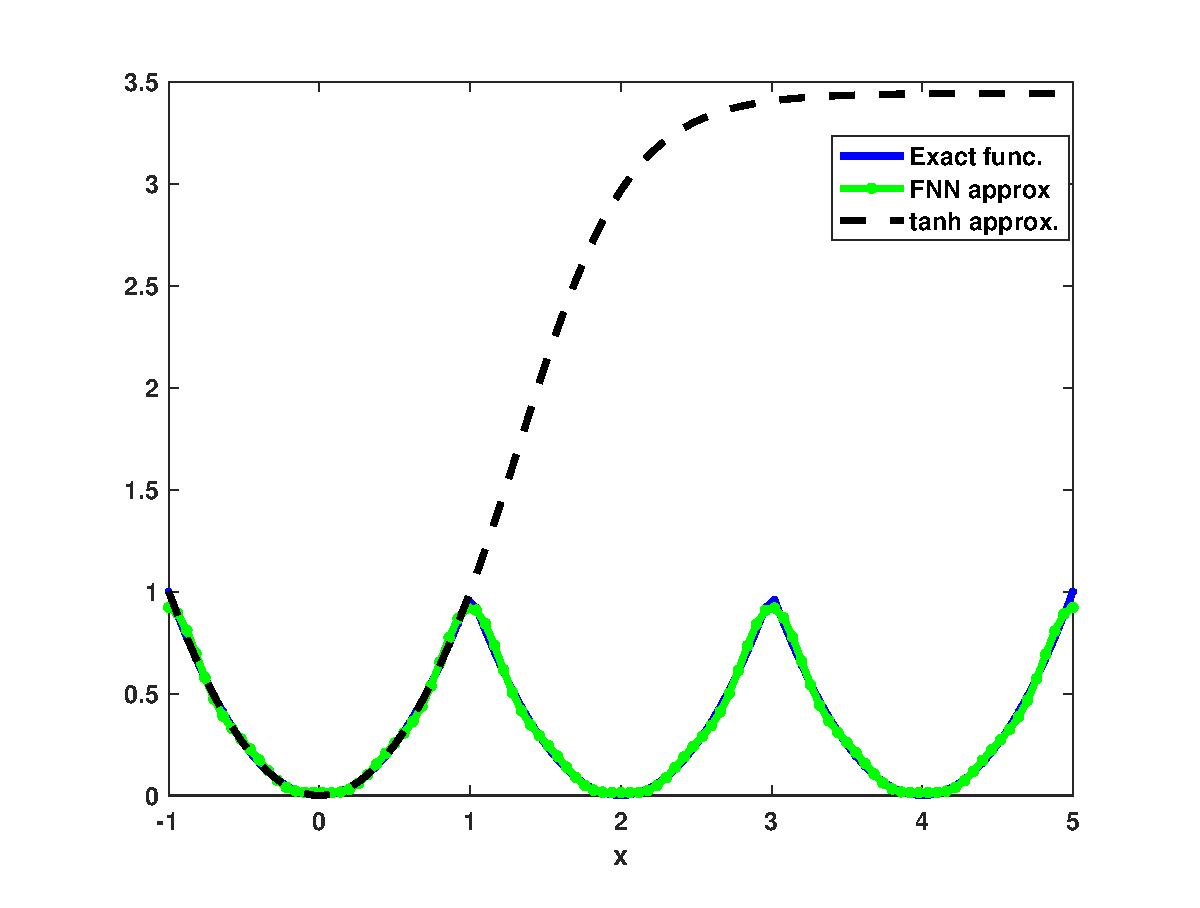
\includegraphics[width=.45\textwidth]{fnnvstanhoutx2.eps}
    \caption{\;Comparison between the FNN and the $\tanh$ approximations outside the training domain for $f(x) = x^2$ }
    \label{fig:Fnnx2out}
\end{figure}
%   \begin{figure}[!htb]
%     \centering
%     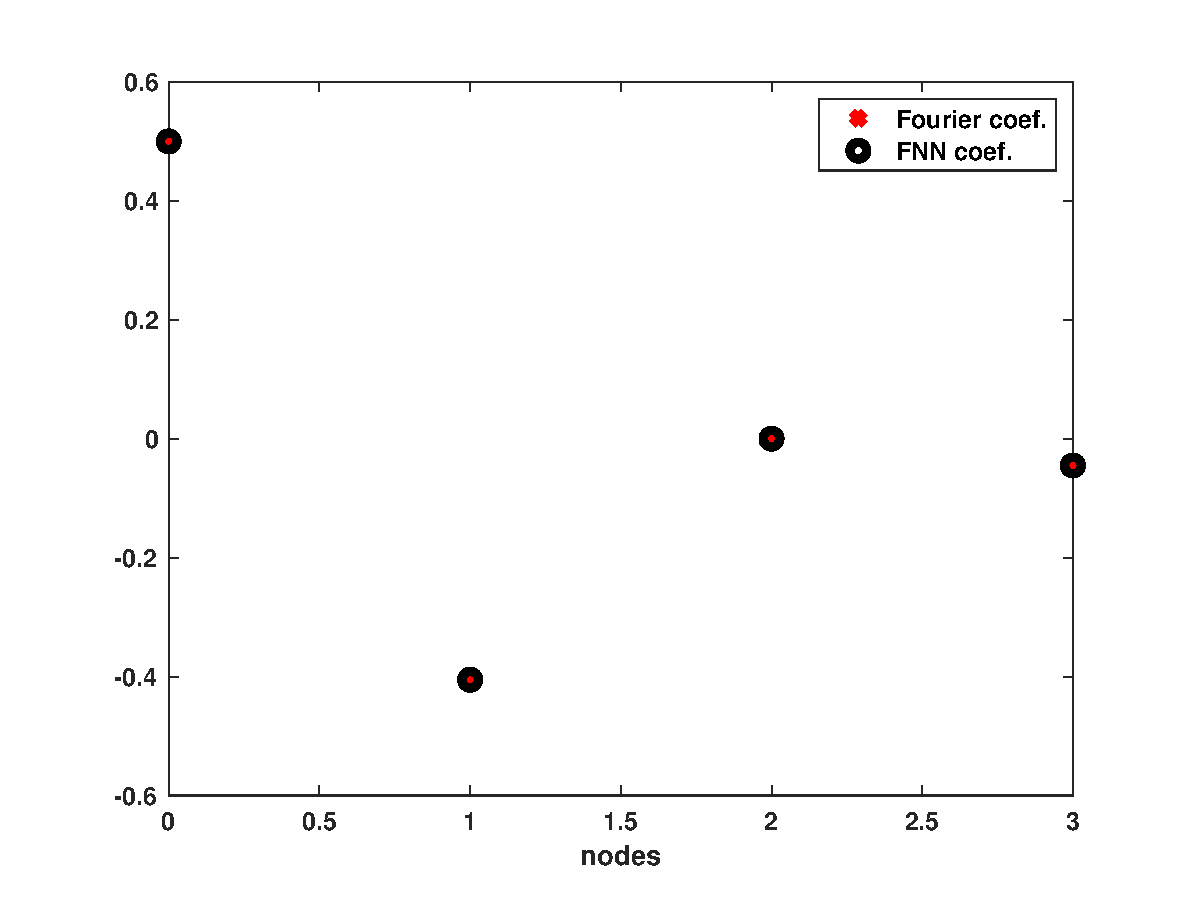
\includegraphics[width=.6\textwidth]{fnncoeffvsfourcoeffabsx.eps}
%     \caption{Comparison between the FNN coefficients and the Fourier coefficients of $f(x) = |x|$ for the $4$ nodes captured by the neural network}
%     \label{Fnnabsx}
% \end{figure}

To conclude the numerical tests in this section, we approximate the function
\begin{equation}\label{Eq:absx}
 g(x) = |x|, \;\; \text{$x \in \left(-(2k+1), (2k+1)\right)$}\;\;, k \in \mathbf{N}   
\end{equation}


The Fourier series of this function is
$$
S(g)(x)= \frac{1}{2} + \sum_{n=1}^{\infty} -4 \frac{(1}{\pi^2 (2n - 1)} \cos(\pi (2n - 1)x)
$$

We summarize the FNN coefficients in table (\ref{tab:tabfnnx2}) as well as the biases produced by the FNN. The FNN was able to capture the first $4$ nodes of the Fourier decomposition. This can be explained by the fact $g$ only admits odd nodes. As before, we provide in figure (\ref{fig:Fnnx2}) (right) a visual representation to compare the Fourier coefficients of $g$ to its FNN coefficients. Similar results to those obtained for the function $f$ (\ref{Eq:xsquare}) are observed here.  The FNN coefficients are good approximations of their Fourier counterparts and the error between the two is of the $3rd$ order.\\
\begin{table}[!h]
  \begin{center}
  \begin{tabular}{ |c|c|c|c|c| } 
    \hline
\multicolumn{3}{|c|}{Number of iterations}& $445$  \\
\hline
  \multicolumn{3}{|c|}{Loss Function (upon convergence)} & $1e-2$  \\
\hline
\hline
$w_k$ & $\phi_k$ & $\lambda_k$& $\phi_0$ \\
\hline
$ 0.99995402$ & $-2.44738021e-03$ &$-0.40420162$& \\ 
$2.98845687$&$-1.68031025e-01$ & $0.03295792$& $0.502531$ \\ 
$2.99445216$& $-6.78306499e-02$ & $-0.07711458$& \\ 
$ -1.99075052$& $-9.45244148$ & $ -0.00391551$& \\ 
\hline
\end{tabular}
\caption{\;Number of iterations, value of the loss function at convergence and optimal weights and biases of the FNN to approximate $ f(x) = |x|$ on $[-1, 1$]}\label{tab:tabfnnx2}
\end{center}
\end{table}


\section{Fourier neural networks as differential equations solvers}\label{sec:fnnpde}
The use of Machine Learning (ML) in the field of differential equations has raised considerable and widespread interest in recent years. ML techniques have been used to effectively solve differential equations \cite{Dockhorn2019}, \cite{hsieh2019learning}, \cite{raissi2017hidden}, \cite{raissi2019Pinn},  and \cite{Sirignano2018} but also to discover underlying dynamics from data \cite{Brunton2016}, \cite{Raissi2018} and \cite{ Rudy2017}  and even to build robust neural networks architectures based on differential equations \cite{Chen2018}, \cite{Long2018} and \cite{Ruthotto2019} . In this section, we extend the work presented in section \ref{sec:fnn} to seek periodic solutions of differential equations of the type $$Pu = f$$ where $P$ is a differential operator. To that aim, we follow \cite{Raissi2018} and \cite{Sirignano2018}  and use the loss function
\begin{equation}\label{Eq:lossfunPDE}
     L(\phi, w, \lambda) = ||P \hat{u}(x) - f(x) ||_2^2  + \alpha_2||\lambda||_2^2 + \alpha_3||w||_2^2 + \alpha_3\left( ||\hat{u}(x + T) - \hat{u}(x)||_2^2\right) + \alpha_4\left( ||\hat{u}(x - T) - \hat{u}(x)||_2^2 \right)
\end{equation}
that incorporates the physics into the loss function to obtain what we call a Physics Informed Fourier Neural Network (PIFNN). This name is inspired by the one introduced in \cite{raissi2019Pinn}. We illustrate the performance of the PIFNN by solving the one-dimensional Poisson and heat equations.

\subsection{Poisson equation}
First, we solve the Poisson equation
\begin{equation}\label{Eq:Poissoneq}
    -\Delta u = \cos(\pi x),\;\;\; x \in [-1,1].
\end{equation}
with the constructed PIFNN. To assess the quality of the PIFNN solution, we compare it to the exact solution of this equation which is given by $u = \frac{1}{\pi^2}\cos(\pi x)$. We show both solutions in figure (\ref{fig:FNNvsexactPoisson}) and we report the weights and biases of the PIFNN in table (\ref{tab:tabPoisson}) . We note that the output is 
$$\hat{u}(x) = -\frac{1}{\pi^2}\cos(\pi x + \pi) + o(1e-5) \approx \frac{1}{\pi^2}\cos(\pi x).$$
which is a $5$th order approximation of the exact solution. We obtain an additional advantage of the PIFNN when seeking periodic solutions of the Poisson equation. In fact, it produces a closed formula for this equation and the exact one csn be retrieved from it.


  \begin{figure}[!htb]
    \centering
    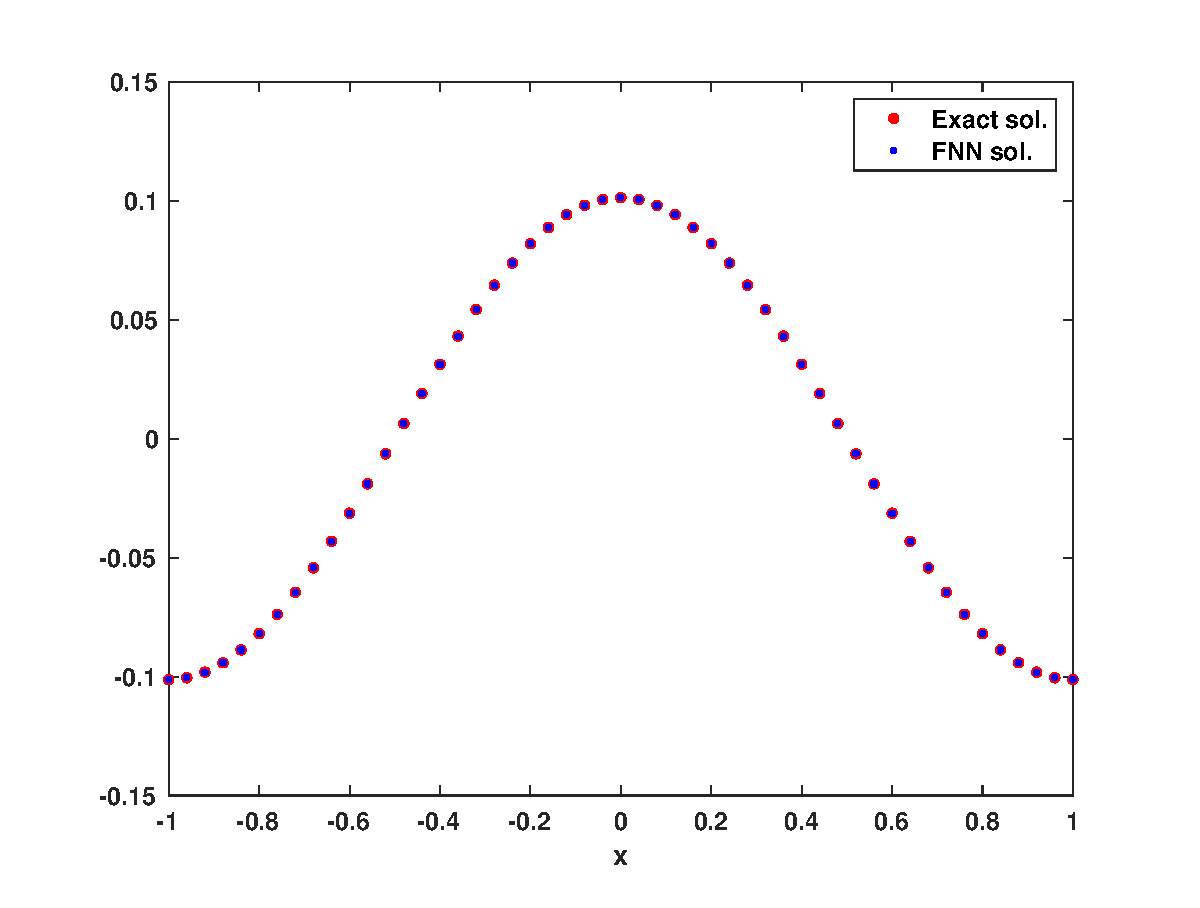
\includegraphics[width=.45\textwidth]{poisson_exvsFNNL2.eps}
    \caption{\;Comparison between the PIFNN and the exact solutions}
    \label{fig:FNNvsexactPoisson}
\end{figure}

 \begin{table}[!h]
  \begin{center}
\begin{tabular}{ |c|c|c|c|c| } 
\hline
$w_k$ & $\phi_k$ & $\lambda_k$& $\phi_0$ \\
\hline
$-3.77424453e-10$ & $-4.42730681$ &$4.90842033e-05$& \\ 
$-1.16548318e-10$&$ 2.46210794$ & $-1.45660922e-05$& $0$ \\ 
$1.00000000$& $ 3.14159265 \approx \pi$ & $-1.01321184e-01 \approx -1/\pi^2$& \\ 
$ -1.18183192e-09$& $ 0.79153364 $ & $-1.60990031e-06$& \\ 
\hline
\end{tabular}
\caption{\;Optimal weights and biases of the FNN to solve the Poisson equation (\ref{Eq:Poissoneq}), $k = 1\cdots4$ }\label{tab:tabPoisson}
\end{center}
\end{table}




\subsection{Heat equation}
Here, we solve the heat equation 
\begin{align}\label{Eq:Heateq}
    \frac{\partial u}{\partial t} &= \frac{\partial^2 u}{\partial^2 x},\;\;\;\;\;\;\;\;\;\;\;\;\;\;\;\;\;\;\;\;\;\;\;\;\; \;x \in [-1,1], \; \;t \in [0,4] \nonumber \\
    u(0,x) &= u_0(x) = \sin(\pi x),\\
    u(t, -1) &= u(t, 1) \nonumber
\end{align}

 \begin{figure}[!htb]
    \centering
    \subfigure{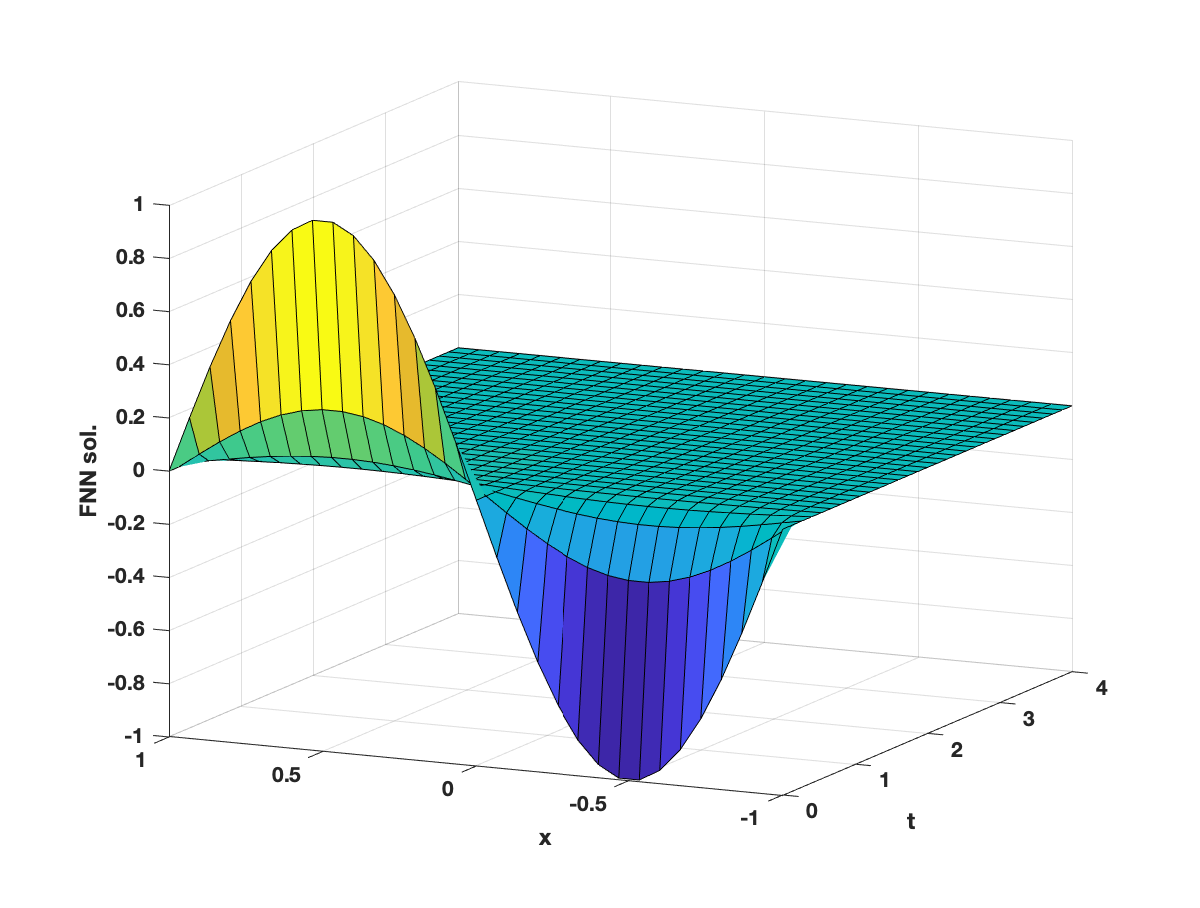
\includegraphics[width=0.45\textwidth]{solfnnheat.eps}}
     \subfigure{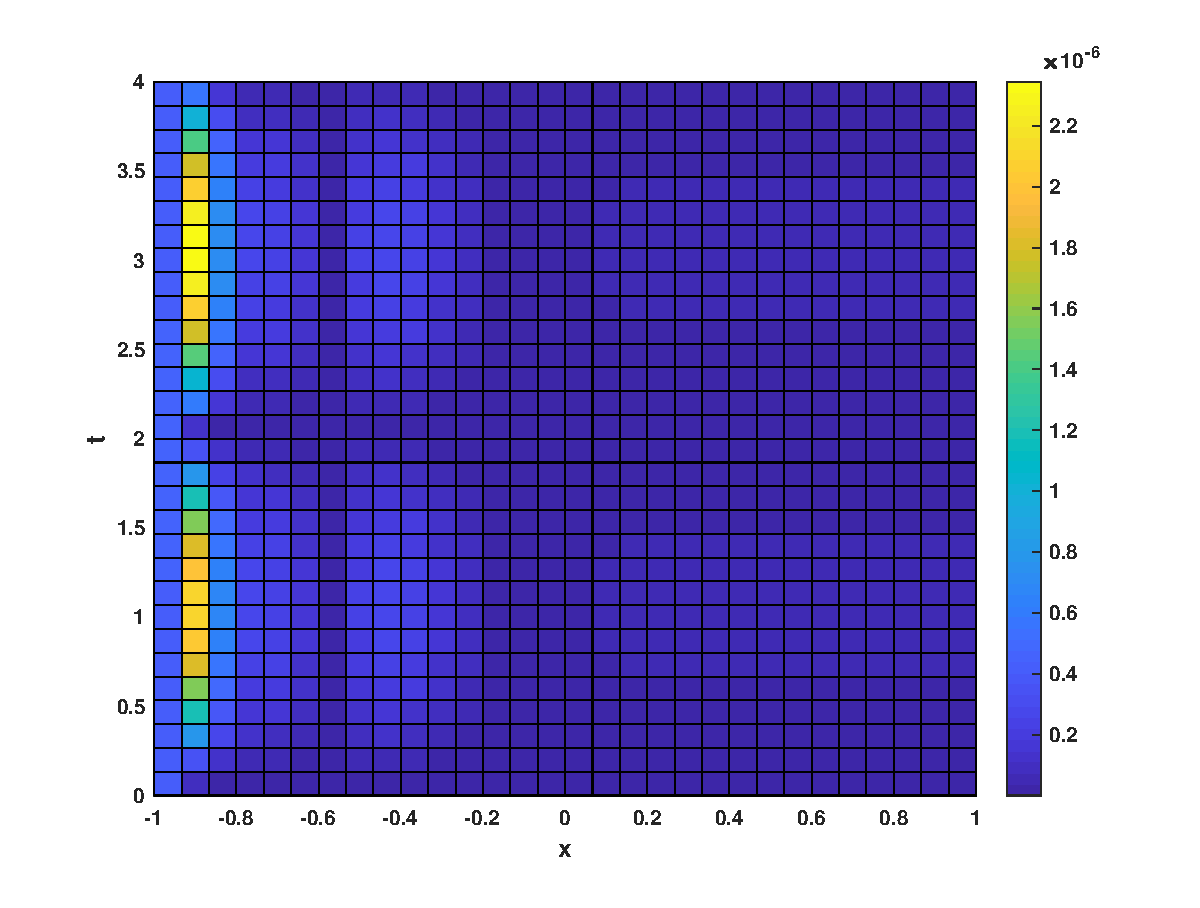
\includegraphics[width=0.45\textwidth]{error_pcolor_heat.eps}}
    \caption{\;Solution produced by the PIFNN for the heat equation (left) and error from the exact solution (right) }
    \label{fig:fnnvsexactheat}
\end{figure}
To account for the time dependency, we rewrite the heat equation using the separation of variables method. To this end, we set $u(x,t) = X(x)T(t)$ which transforms the equation into 
$$X(x)T'(t) = X''(x)T(t).$$
We rewrite the cost function as follows 
\begin{align*}
    L(\phi, w, \lambda) &= \alpha_1||\hat{X}(x)\hat{T}'(t)-\hat{X}''(x)\hat{T}(t)||^2  \\ &+\alpha_2||\lambda||^2 + \alpha_3||w||^2 \\ 
    &+\alpha_3 ||\hat{X}(x + 2) - \hat{X}(x)||^2 \\
    &+\alpha_4||\hat{X}(x - 2) - \hat{X}(x)||^2  \\
   &+ \alpha_5||\hat{T}_0(x) - \hat{u}_0(x)||^2
\end{align*}
to incorporate the boundary and initial conditions and separate the network into two independant subnetworks. The first with the PIFNN architecture that deals with the space dependent function $X$ and second with a regular architecture (with a $\tanh$ activation function) that works on the time dependent function $T$. The left part of figure (\ref{fig:fnnvsexactheat}) corresponds the solution produced by the PIFNN and the right part shows the error between that solution and the exact one which is $$u(x) = \sin(\pi x)e^{-\pi^2 t}, \;\; t \in [0,4]$$. We note from the figure that error between the two is of order $6$. \\
% Finally, we solve the following system of differential equations obtained from \cite{Teschl2012} 
% \begin{align}
%     \frac{\partial x_1}{\partial t} &= -\pi  x_2 + x_1(1 - x_1^2 - x_2^2) \nonumber \\ 
%     \frac{\partial x_2}{\partial t} &= \pi  x_1 + x_2(1 - x_1^2 - x_2^2) \\
% \end{align}\label{sys_per}
% This system admits a periodic solution given by $u(t)=(cos(\pi t), sin(\pi t))$


%\section{Results}



\section{Conclusion}
We have constructed a novel Fourier Neural Network (FNN) architecture that successfully approximates low-frequency analytic and piecewise analytic one dimensional periodic functions. We were able to retrieve the Fourier coefficients for such functions with third order accuracy. We also showed how to seek periodic solutions for simple one dimensional differential equations. These results were achieved by imposing periodicity constraints to the optimization problem we are solving and by subsequently solving the problem with a penalty-like method. Besides significantly improving the results obtained using traditional neural networks in terms of accuracy and number of iterations, our simulations revealed another important advantage, namely, it conserves the properties of the learned task (approximating a function etc) outside of the training domain. One limitation of our model is that we are not using a rigorous technique for picking the penalty coefficients but are instead setting them up by trial and error. Another limitation is that we need to know the periodicity of the function we are estimating a priori in order to incorporate it in the activation function. We are currently in the process of investigating solutions to overcome these limitations. Our results are promising and we are planning on extending to multidimensional functions in future work. We believe the framework presented here can serve as a preprocessing tool for many engineering and scientific applications such as electronics, image recognition and acoustics where the Fourier decomposition is widely used.


\section*{Acknowledgement}
 The authors would like to thank Charlotte Haley for her pertinent suggestions. This material is based upon work supported by the
U.S. Department of Energy, Office of Science, Advanced Scientific
Computing Research under Contract DE-AC02-06CH11357. 
{\bf Government License.}  The submitted manuscript has been created by
UChicago Argonne, LLC, Operator of Argonne National Laboratory
(``Argonne''). Argonne, a U.S. Department of Energy Office of Science
laboratory, is operated under Contract No. DE-AC02-06CH11357. The
U.S. Government retains for itself, and others acting on its behalf, a
paid-up nonexclusive, irrevocable worldwide license in said article to
reproduce, prepare derivative works, distribute copies to the public,
and perform publicly and display publicly, by or on behalf of the
Government.  The Department of Energy will provide public access to
these results of federally sponsored research in accordance with the
DOE Public Access
Plan. http://energy.gov/downloads/doe-public-access-plan.
\appendix
\section{Some statistical properties}\label{appendixA}
We recall below some properties verified by the mean $\mu$ and the variance $\sigma^2$ of a random variable.
\begin{enumerate}[label=Property \arabic*.,itemindent=*]
  \item $\mu(aX + Y) = a\mu(X) + \mu(Y)$ and $\sigma^2(aX+Y) = a^2\sigma^2(X) + \sigma^2(Y)$ where $a \in \mathbf{R}$, and $X$ and $Y$ are two random variables,
  \item $\mu(XY) = \mu(X) \mu(Y)$ and $\sigma^2(XY) = \sigma^2(X) \left(\mu^2(Y) + \sigma^2(Y)\right) + \mu^2(X)\sigma^2(Y)$ where $X$ and $Y$ are two independent random variables,
\end{enumerate}
We also recall the value of the mean and of the variance of the two distributions used in the paper i.e the uniform and normal distributions. 
\begin{enumerate}
  \item If $X \sim \mathcal{U}([a,b])$ then:
  \begin{itemize}
      \item $\mu(X) = \frac{1}{b - a}$ and  $\sigma^2(X) = \frac{(b - a)^2}{12} $,
      \item The  probability density function (pdf) of $X$ is $f_X(x) = 1/(b-a)$ if $x \in [a,b]$ and $0$ otherwise
  \end{itemize}
   
  \item If $X \sim \mathcal N (0, m^2)$ then:
   \begin{itemize}
      \item $\mu(X) = 0$ and  $\sigma^2(X) = m^2$, 
      \item The  probability density function (pdf) of $X$ is $f_X(x) = \frac{1}{\sigma \sqrt{2\pi}}e^{-\frac{x^2}{2\sigma^2}}$
  \end{itemize}
\end{enumerate}




















\bibliographystyle{plain}
\bibliography{MLFNN}



%  \section*{Authors Biographies}

%  \begin{biography}{
\includegraphics[width=60pt,height=70pt,draft]{empty}}{\textbf{Marieme Ngom.} Marieme received her PhD degree in applied mathematics from the University of Illinois at Chicago and is currently a postdoctoral researcher in the Mathematics and Computer Science (MCS) division of Argonne National Laboratory. Her research interests include numerical methods for partial Differential Equations and high performance computing.}
%  \end{biography}
%  \begin{biography}{
\includegraphics[width=60pt,height=70pt,draft]{empty}}{\textbf{Oana Marin} Oana received her PhD from the KTH Royal Institute of Technology. During her studies, she developed numerical methods to handle the singular kernels arising in boundary integral formulations of the Stokes and Laplace equations. She has also worked on numerical methods of simulating efficiently large-scale suspensions of particles/fibers.}
%  \end{biography}


\end{document}
